\documentclass[conference]{IEEEtran}
\IEEEoverridecommandlockouts

% --- Packages ---
\usepackage{cite}
\usepackage{amsmath,amssymb,amsfonts}
\usepackage{graphicx}
\usepackage{textcomp}
\usepackage{xcolor}
\usepackage{booktabs}
\usepackage{tabularx}
\usepackage{array}
\usepackage{float}
\usepackage[hidelinks]{hyperref}
\usepackage[section]{placeins}

% Shrink wide tables to text width; leave narrow tables at natural size.
\newcommand{\maxwidthtable}[1]{%
  \resizebox{\ifdim\width>\linewidth \linewidth\else \width\fi}{!}{#1}%
}

% Loosen IEEE float defaults so the per-subsection FloatBarrier above does not
% leave half-empty pages: allow nearly-empty float pages and tiny text fragments.
\renewcommand{\topfraction}{0.95}
\renewcommand{\bottomfraction}{0.8}
\renewcommand{\textfraction}{0.05}
\renewcommand{\floatpagefraction}{0.5}
\renewcommand{\dbltopfraction}{0.95}
\renewcommand{\dblfloatpagefraction}{0.5}
\setcounter{topnumber}{4}
\setcounter{bottomnumber}{3}
\setcounter{totalnumber}{6}
\setcounter{dbltopnumber}{4}

\begin{document}

% --- Title ---
\title{Parameter-Efficient Adaptation of SAM~2 for Sentinel-1 SAR Flood Inundation Mapping in the Indo-Gangetic Region}

\author{
\IEEEauthorblockN{Aksan Gony Alif}
\IEEEauthorblockA{\textit{Department of Computer Science and Engineering} \\
\textit{BRAC University}\\
Dhaka, Bangladesh}
\and
\IEEEauthorblockN{Mahbubur Rahman}
\IEEEauthorblockA{\textit{Department of Computer Science and Engineering} \\
\textit{BRAC University}\\
Dhaka, Bangladesh}
}

\maketitle

% --- Abstract ---
\begin{abstract}
Bangladesh experiences large-scale monsoon flooding almost every year, and monsoon-season cloud cover renders optical satellite imagery unreliable precisely when flood mapping is most urgent. Synthetic Aperture Radar (SAR) imagery from Sentinel-1 is the operational alternative because radar penetrates clouds, but its noisy single-channel intensity statistics differ fundamentally from the natural RGB photographs on which modern vision foundation models are pretrained. We present a parameter-efficient adaptation of the Segment Anything Model 2 (SAM~2) to Sentinel-1 SAR flood inundation mapping that addresses three gaps in prior work. First, no published peer-reviewed paper has compared competing parameter-efficient fine-tuning (PEFT) methods on SAM-family backbones for SAR flood segmentation: we run a head-to-head comparison of LoRA, DoRA, Convolutional LoRA, and AdaptFormer on two SAM-family backbones (SAM ViT-B and SAM~2 Hiera-Base-Plus) across three seeds, plus three larger stretch backbones (SAM ViT-L, SAM ViT-H, SAM~2 Hiera-Large) under Conv-LoRA, and surface a substantive trade-off in which AdaptFormer maximizes in-distribution IoU while the LoRA family is more robust on held-out countries. Second, prior SAR-flood uncertainty work reports low Expected Calibration Error but does not test whether per-pixel scores rank pixels by difficulty: we evaluate Monte Carlo dropout with both aggregate calibration and a pointwise selective-prediction analysis, finding that the two need not agree on out-of-distribution (OOD) events, with aggregate calibration holding while selective-prediction curves stay flat. Third, no released SAM-evaluation surface combines temporal and geographic OOD shift on a public reproducible Sentinel-1 acquisition: we contribute a Pakistan-2022 SAR flood test set (39 chips at Sentinel-1's native 10\,m resolution) built by pairing TU Wien Sentinel-1-derived flood-extent labels with Microsoft Planetary Computer Sentinel-1 imagery through a documented pipeline. A polarimetric ablation that varies how the two Sentinel-1 polarization channels are composed into a three-channel input localizes the Pakistan-2022 OOD failure mode to the cross-polarization (VH) channel itself: removing VH and feeding only the co-polarization (VV) channel raises SAM-family Pakistan-2022 IoU roughly six-fold (from $0.09$--$0.14$ to $0.56$--$0.66$, $\pm$ one standard deviation across three seeds), landing within $0.01$ to $0.12$ IoU of the U-Net baseline at $0.672$. The full experimental sweep (five backbones, four PEFT methods, three seeds, polarimetric ablations, U-Net and zero-shot baselines) completes in approximately 3.5 hours on a dual NVIDIA RTX PRO 5000 Blackwell cloud instance for under ten US dollars of cloud compute.
\end{abstract}

\begin{IEEEkeywords}
Segment Anything Model, parameter-efficient fine-tuning, synthetic aperture radar, flood inundation mapping, foundation models, confidence-aware learning, Indo-Gangetic Plain, Pakistan, Bangladesh.
\end{IEEEkeywords}

% --- 1. Introduction ---
\section{Introduction}
\label{sec:intro}

Floods are among the most damaging natural disasters worldwide, and their economic and humanitarian costs have risen sharply over the past two decades as a consequence of climate change, accelerated urbanization in flood-prone regions, and the increasing frequency of extreme precipitation events~\cite{Hu2025GlobalFloods}. Bangladesh, situated on the alluvial plains of the Ganges, Brahmaputra, and Meghna river systems, is particularly exposed. During a typical monsoon season, between twenty and twenty-five percent of the country's land area becomes inundated; during severe events the figure has historically reached between thirty and sixty percent. The 2022 Sylhet flash flood affected approximately 7.2 million people across nine northeastern districts and displaced an estimated 480{,}000 people at the peak of the event. Accurate, timely flood-extent mapping is an operational humanitarian requirement.

The dominant remote sensing modality for global flood monitoring is the European Space Agency's Sentinel-1 mission, which provides free Synthetic Aperture Radar (SAR) imagery at ten-meter resolution with a six-day revisit time. SAR dominates over optical alternatives because radar wavelengths penetrate clouds: during the South Asian monsoon, cloud cover over Bangladesh routinely exceeds eighty percent for weeks at a time. However, SAR imagery differs fundamentally from the natural RGB photographs on which contemporary vision foundation models are trained. SAR is dual-polarization, expressed in decibels on a logarithmic scale, and dominated by multiplicative speckle noise rather than additive Gaussian noise.

The Segment Anything Model (SAM)~\cite{Kirillov2023SAM} and its successor SAM~2~\cite{Ravi2025SAM2} have raised a natural question: can these models be adapted to SAR data, and what is the right adaptation strategy given limited compute? Full fine-tuning is impractical even for the smallest variants, but parameter-efficient fine-tuning (PEFT) techniques such as Low-Rank Adaptation~\cite{Hu2022LoRA}, Weight-Decomposed Low-Rank Adaptation~\cite{Liu2024DoRA}, Convolutional LoRA~\cite{Zhong2024ConvLoRA}, and AdaptFormer~\cite{Chen2022AdaptFormer} can match or approach full fine-tuning at a fraction of the cost.

Three substantive gaps in prior work motivate this paper (detailed in Section~\ref{sec:related}): no head-to-head comparison of PEFT methods on SAM-family backbones for SAR flood segmentation; no evidence that aggregate-level calibration of confidence-aware estimators translates to operationally useful per-pixel uncertainty on out-of-distribution flood events; and no released SAM-evaluation surface combining temporal and geographic out-of-distribution shift on a public Sentinel-1 acquisition. We address them through four research questions. Which PEFT method is most effective, and is the best in-distribution method also the most generalization-robust? Does polarimetric composition of the dual-polarization signal materially affect accuracy? Can a Monte Carlo dropout confidence-aware mechanism deliver calibrated per-pixel uncertainty that is also operationally useful for selective prediction on held-out events? How well do the adapted models generalize from a globally diverse training distribution to a strictly held-out country and a future flood event? The principal contributions are a systematic empirical comparison of four PEFT methods on two SAM-family backbones against a U-Net baseline and zero-shot baselines (Section~\ref{sec:results-headline}), a polarimetric prompt-engineering ablation establishing a defensible pseudo-RGB composition convention for dual-polarization Sentinel-1 input (Section~\ref{sec:results-polari}), and a Monte Carlo dropout confidence-aware mechanism evaluated both at aggregate-calibration level and at pointwise-utility level (Sections~\ref{sec:results-confidence} and~\ref{sec:results-selective}). A fourth artifact, a custom Pakistan-2022 SAR flood test set constructed from TU Wien flood-extent labels and Microsoft Planetary Computer Sentinel-1 imagery, is built in this work and used as a strict out-of-distribution evaluation surface (Section~\ref{sec:datasets}).

% --- 2. Related Work ---
\section{Related Work}
\label{sec:related}

\subsection{Vision Foundation Models and the Segment Anything Family}

SAM~\cite{Kirillov2023SAM} comprises a Vision Transformer (ViT) image encoder, a prompt encoder, and a lightweight mask decoder, trained on the SA-1B dataset of over one billion masks. SAM~2~\cite{Ravi2025SAM2}, presented as an Oral at ICLR 2025, replaces the plain ViT encoder with a Hiera architecture (a hierarchical transformer that produces multi-scale features rather than a single token grid) and adds a streaming memory module for video. For still-image flood mapping, the multi-scale Hiera encoder is the consequential change; the memory module is not used in this work. The released SAM~2 variants span Hiera-Tiny (39M), Hiera-Small (46M), Hiera-Base-Plus (81M), and Hiera-Large (224M). Of particular relevance to non-RGB adaptation, MedSAM~\cite{Ma2024MedSAM} demonstrated that SAM's pretrained features transfer to medical imaging when full fine-tuned on a curated mask corpus.

\subsection{Parameter-Efficient Fine-Tuning}

LoRA~\cite{Hu2022LoRA} approximates the weight update during fine-tuning as a low-rank decomposition $\Delta W = BA$ with $B \in \mathbb{R}^{d\times r}$, $A \in \mathbb{R}^{r\times d}$ and $r \ll d$, training only $A$ and $B$ while freezing the pretrained $W$. DoRA~\cite{Liu2024DoRA} refines LoRA by decomposing $W$ into a magnitude vector and a directional matrix, applying low-rank updates only to the direction. Convolutional LoRA~\cite{Zhong2024ConvLoRA} augments LoRA with ultra-lightweight depthwise convolutions on the low-rank intermediate, injecting locality-aware inductive bias into a plain ViT encoder. AdaptFormer~\cite{Chen2022AdaptFormer} inserts parallel bottleneck adapter modules into each transformer's feed-forward block.

\subsection{SAM Adaptation for Remote Sensing and SAR}

ClassWise-SAM-Adapter (CWSAM)~\cite{Pu2025CWSAM} is the closest prior work: it freezes most of SAM's parameters, inserts lightweight adapters into the encoder, and adds a class-aware mask decoder for multi-class SAR landcover segmentation. CWSAM targets landcover classification rather than flood mapping; the present work extends the methodological frame to flood inundation, evaluates SAM~2 in addition to SAM, includes a confidence-aware mechanism, and reports on a 2022 Pakistan out-of-distribution test set.

\subsection{SAR Flood Mapping with Deep Learning}

Sen1Floods11~\cite{Bonafilia2020Sen1Floods11} is the canonical benchmark dataset for Sentinel-1 SAR flood mapping. DAM-Net~\cite{Saleh2024DAMNet} reports F1 above 96\% and IoU above 93\% on the S1GFloods benchmark using a Siamese ViT with differential attention. DeepSARFlood~\cite{Sharma2025DeepSARFlood} achieves an IoU of 0.72 on Sen1Floods11 using a deep ensemble of ViT/CNN-ViT hybrids and reports uncertainty estimates derived from ensemble disagreement. The PANGAEA benchmark~\cite{Marsocci2024PANGAEA} establishes that a vanilla 30M-parameter U-Net often matches or exceeds large geospatial foundation models on Sen1Floods11, which motivates the explicit U-Net baseline in this paper.

\subsection{Research Gap}

Three substantive gaps remain in the intersection of foundation-model adaptation, SAR flood mapping, and uncertainty estimation that this paper addresses.

\textit{Gap 1: No systematic PEFT comparison on SAM for SAR.}~CWSAM~\cite{Pu2025CWSAM} adapts SAM with a single adapter design for SAR landcover classification, and parameter-efficient methods such as LoRA, DoRA, Conv-LoRA, and AdaptFormer have been benchmarked on natural-image segmentation and medical imaging~\cite{Hu2022LoRA,Liu2024DoRA,Zhong2024ConvLoRA,Chen2022AdaptFormer,Ma2024MedSAM}, but no published peer-reviewed work has performed a head-to-head comparison of competing PEFT methods on SAM-family backbones for Sentinel-1 SAR flood segmentation. The trade-offs that determine the right adapter for this domain, in particular the trade-off between in-distribution accuracy and out-of-distribution generalization, are therefore undocumented.

\textit{Gap 2: Aggregate calibration may not imply operationally useful per-pixel uncertainty on out-of-distribution data.}~Prior SAR-flood uncertainty work derives uncertainty from ensemble disagreement~\cite{Sharma2025DeepSARFlood} and reports aggregate calibration metrics, but does not test whether the resulting per-pixel uncertainty scores correctly rank pixels by difficulty on strictly held-out flood events. Practitioners deploying SAR-flood models in operational humanitarian pipelines need to know whether MC-dropout (or any aggregate-calibrated estimator) can be used to abstain on hard pixels, which this paper tests directly.

\textit{Gap 3: No SAM-evaluation surface combining temporal and geographic OOD on a public, reproducible SAR flood acquisition.}~Sen1Floods11~\cite{Bonafilia2020Sen1Floods11} provides global geographic diversity but its events are all from 2017--2019. The TU Wien Pakistan-2022 flood-extent product~\cite{Roth2023Pakistan} is released as labels only; pairing it with Sentinel-1 imagery for foundation-model evaluation requires an explicit acquisition pipeline that has not been released alongside any SAM-family adaptation paper.

The present paper fills all three gaps: a four-by-two PEFT-by-backbone matrix at three seeds with stretch backbones (Sections~\ref{sec:results-headline} and~\ref{sec:results-stretch}); a Monte Carlo dropout uncertainty analysis spanning aggregate calibration (Section~\ref{sec:results-confidence}) and pointwise selective prediction (Section~\ref{sec:results-selective}); and a 39-chip Pakistan-2022 test set at Sentinel-1's native 10-metre resolution, built from TU Wien labels paired with Microsoft Planetary Computer Sentinel-1 RTC imagery via a documented pipeline.

% --- 3. Methodology ---
\section{Methodology}
\label{sec:methodology}

\subsection{Backbone Selection}

Five backbones are evaluated. The principal pair is SAM ViT-B (\textasciitilde 94M total parameters), the canonical baseline used by nearly every SAM adaptation paper in the literature, and SAM~2 Hiera-Base-Plus (\textasciitilde 81M, matching the count reported in Section~\ref{sec:related}), the primary novel-contribution backbone with multi-scale features through the Hiera architecture and a streaming memory module. The three stretch backbones, evaluated under Conv-LoRA only, are SAM ViT-L (\textasciitilde 308M), SAM ViT-H (\textasciitilde 636M) and SAM~2 Hiera-Large (\textasciitilde 224M). All five fit within the 48~GB VRAM budget of the RTX PRO 5000 Blackwell used for the cloud sweep.

\subsection{Parameter-Efficient Fine-Tuning Methods}

Four methods are compared under a common training protocol:
\begin{itemize}
\item \textbf{LoRA}: $\Delta W = (\alpha/r) BA$ on the fused QKV and output projections of every transformer block. Rank $r = 8$, initialization Kaiming-uniform for $A$ and zero for $B$.
\item \textbf{DoRA}: as LoRA but with the magnitude/direction decomposition; trained magnitude vector initialized to the base weight column norms.
\item \textbf{Convolutional LoRA}: LoRA augmented with a $3 \times 3$ depthwise convolution on the low-rank intermediate, reshape-aware so the spatial layout of tokens is preserved.
\item \textbf{AdaptFormer}: parallel bottleneck adapter on each FFN block; bottleneck width 64, scale parameter initialized to one and up-projection initialized to zero (the side-path emits zero at init but its up-projection gradient is non-zero, so the adapter can begin learning immediately; setting both to zero freezes the path, an init-bug we discuss in Section~\ref{sec:discussion}).
\end{itemize}
For all four methods, the prompt encoder is frozen and the mask decoder is augmented with LoRA rank-4 adapters on all linear layers, providing a consistent low-rank decoder adaptation across methods. Implementations follow the reference equations from~\cite{Hu2022LoRA}, \cite{Liu2024DoRA}, \cite{Zhong2024ConvLoRA}, and~\cite{Chen2022AdaptFormer}.

\subsection{Polarimetric Prompt Engineering}

Sentinel-1 imagery is dual-polarization: a co-polarized channel VV (vertical transmit, vertical receive) and a cross-polarized channel VH (vertical transmit, horizontal receive). SAM~2, however, was pretrained on three-channel RGB photographs, so adapting it to SAR requires synthesizing a third channel from the two available polarizations (a ``pseudo-RGB'' composition). We compare three compositions: (1) $\text{ratio}: (\text{VV}, \text{VH}, \text{VV}-\text{VH})$ in dB, with the third channel a log-domain ratio; (2) $\text{diff}$: same structurally but framed as VV-minus-VH; (3) $\text{single}$: VV replicated across all three channels, as a single-polarization control. All compositions are followed by 2nd/98th percentile clipping and per-channel z-score normalization with statistics computed once on the Sen1Floods11 training split and held fixed thereafter.

\subsection{Confidence-Aware Mechanism}

We adopt Monte Carlo (MC) dropout as the confidence-aware variant. At inference, dropout layers in the mask decoder remain active and twenty independent forward passes are run per chip. The mean of the resulting sigmoid probabilities is the prediction; the per-pixel standard deviation is the epistemic uncertainty estimate. Calibration is reported via expected calibration error (ECE) computed with 15 equal-width probability bins following Guo~\textit{et al.}, and visualized as a reliability diagram.

% --- 4. Datasets ---
\section{Datasets}
\label{sec:datasets}

The principal in-distribution dataset is Sen1Floods11~\cite{Bonafilia2020Sen1Floods11}, which provides 446 hand-labeled 512$\times$512 chips across eleven flood events in ten countries. We use the official train/valid/test split (252/89/90 chips) for the principal evaluation and the held-out Bolivia split (15 chips) as the canonical out-of-distribution surface.

To strengthen the regional generalization story, we additionally evaluate on two Pakistan-flavored splits. The first is a country-filtered subset of the Sen1Floods11 hand-labeled chips, comprising the 12 Pakistan chips appearing in the test and valid splits (2010 Pakistan flood event, in-distribution as Pakistan is also in training). The second is a custom Pakistan-2022 test set constructed in this work from two complementary public sources: the Vienna University of Technology (TU Wien) Sentinel-1-derived flood-extent product released alongside~\cite{Roth2023Pakistan} (164 mask tiles at 20-meter resolution on the Equi7Grid Asia coordinate system, an equal-area projection used in the SAR community), and the Microsoft Planetary Computer's \texttt{sentinel-1-rtc} catalogue (Radiometric Terrain Corrected, or RTC, products are pre-georeferenced versions of standard Sentinel-1 Ground Range Detected, or GRD, imagery, queried through the SpatioTemporal Asset Catalog or STAC API). The construction pipeline, packaged as the Pakistan-2022 acquisition pipeline in the released codebase, parses each TU Wien mask filename for the acquisition timestamp and orbit, finds the matching S1 RTC product via STAC search, reads the VV and VH bands lazily over HTTP using rasterio, and tiles the paired imagery and labels into 512$\times$512 chips. To avoid a resolution artifact between Sentinel-1's native 10-metre UTM grid and the TU Wien 20-metre Equi7Grid, the pipeline keeps the Sentinel-1 imagery at its native 10-metre resolution and reprojects the flood masks upward to 10~m via nearest-neighbour; each chip therefore covers $5.12 \times 5.12$~km, matching the Sen1Floods11 training distribution. The August--September~2022 peak-flood window produces 39 chips that satisfy the validity and label-fraction filters. Microsoft Planetary Computer issues anonymous SAS tokens for the \texttt{sentinel-1-rtc} blob storage, so the pipeline runs without account registration.

Table~\ref{tab:datasets} summarizes the four evaluation splits.

\begin{table}[!htbp]
\centering
\caption{The four evaluation splits used in this paper: in-distribution Sen1Floods11, a held-out country (Bolivia), a regional in-distribution Pakistan slice from the 2010 event, and a strictly out-of-distribution Pakistan-2022 set (2022 event, built in this work) that tests generalization to a new event in time as well as geography.}
\label{tab:datasets}
\maxwidthtable{%
\small
\begin{tabular}{lcc}
\toprule
\textbf{Split} & \textbf{Chips} & \textbf{Role} \\
\midrule
Sen1Floods11 test       & 90 & In-distribution (10 countries) \\
Sen1Floods11 Bolivia    & 15 & OOD (only held-out country) \\
Pakistan-S1F11 subset & 12 & Regional in-distribution slice \\
Pakistan-2022 (this work) & 39 & OOD (2022 event) \\
\bottomrule
\end{tabular}%
}
\end{table}

% --- 5. Experimental Setup ---
\section{Experimental Setup}
\label{sec:setup}

\subsection{Hardware and Software}

The full experimental sweep runs on a single rented Vast.ai instance with two NVIDIA RTX PRO 5000 Blackwell graphics processors (48~GB GDDR7 ECC each, 96~GB total) attached to a 64-core host with 503~GB system RAM. Pairs of configurations train concurrently, one per device. The software stack is Python 3.14, PyTorch 2.11 with CUDA 13.0, HuggingFace Transformers 5.9 (the first release with native SAM~2 support), and PyTorch Lightning 2.6. Total wall-clock for the full sweep including the polarimetric ablation, the stretch backbones, the U-Net baseline, the zero-shot baselines, the aggregate evaluation pass and the figure generation is approximately 3.5~hours at marketplace floor pricing of two US dollars per host-hour, for a total cloud cost under ten US dollars.

\subsection{Training Protocol}

Each (backbone, PEFT, seed) configuration is fine-tuned for 10 epochs on the 252 hand-labeled Sen1Floods11 training chips. The optimizer is AdamW with separate learning rates for adapter parameters ($10^{-4}$) and any unfrozen pretrained parameters ($10^{-5}$), weight decay $10^{-2}$, and $\beta = (0.9, 0.999)$. The schedule is a linear warmup over 200 steps followed by cosine decay. The loss is the sum of Dice loss and binary cross-entropy with logits, with equal weighting. Mixed-precision fp16 is used throughout. Batch size is~1 with gradient accumulation~4 (effective batch~4). No training-time data augmentation is applied; the small Sen1Floods11 hand-labeled training set (252 chips) is fed directly through the model. Test-time augmentation (four 90-degree rotations crossed with horizontal flipping, eight views in total) is applied at inference time only for the ensemble + TTA condition reported in Section~\ref{sec:results-ensemble}. Brightness, contrast, and color jitter are not used at either training or test time because they are physically inappropriate for SAR data on a logarithmic decibel scale. Random seeds 42, 123, and 20025 are used for the three reported repetitions.

\subsection{Baselines}

A U-Net with ResNet-34 encoder pretrained on ImageNet (segmentation\_models\_pytorch) is trained from scratch under the same protocol as the principal baseline, motivated by PANGAEA's finding~\cite{Marsocci2024PANGAEA} that a vanilla U-Net often matches large geospatial foundation models on Sen1Floods11. Two zero-shot baselines are also reported: SAM ViT-B and SAM~2 Hiera-Base-Plus with no fine-tuning whatsoever, prompted with a whole-image bounding box. The zero-shot baselines establish a lower bound on what the PEFT adaptation contributes beyond the pretrained features.

% --- 6. Results ---
\section{Results}
\label{sec:results}

\subsection{Headline Comparison Across PEFT Methods and Backbones}
\label{sec:results-headline}

Table~\ref{tab:results_main} reports IoU on each of the four evaluation splits, averaged over three random seeds.

\paragraph{Baselines}
The U-Net baseline establishes the strong simple-architecture reference recommended by PANGAEA~\cite{Marsocci2024PANGAEA}, reaching an in-distribution IoU of $0.601$ on the Sen1Floods11 test split. Zero-shot SAM ViT-B and SAM~2 Hiera-Base-Plus, prompted with a whole-image bounding box and no fine-tuning whatsoever, reach $0.107$ and $0.111$ respectively on the same split, establishing the floor that the PEFT adaptation must improve upon.

\paragraph{In-distribution PEFT comparison}
On SAM~2 Hiera-Base-Plus the four PEFT methods cluster between $0.599$ IoU (LoRA) and $0.634$ IoU (AdaptFormer). AdaptFormer therefore achieves the strongest in-distribution performance, a $0.033$ IoU gain over the U-Net baseline at a fraction of the trainable-parameter cost.

\paragraph{Bolivia held-out country}
The same backbone-method ranking is preserved on the Bolivia out-of-distribution split modulo larger seed variance: DoRA on SAM~2 Hiera-Base-Plus reaches $0.637$ (slightly below the U-Net's $0.684$ but at a small fraction of the U-Net's trainable parameters), while AdaptFormer collapses to $0.458$ IoU under high seed variance ($\pm 0.246$ across three seeds). The Pakistan subset of Sen1Floods11 falls between the in-distribution test and Bolivia as expected for a regional in-distribution slice.

\paragraph{Pakistan-2022 collapse and its cause}
The Pakistan-2022 split, the only strict out-of-distribution test by both geography and time, exposes a far larger separation than the held-out country. The U-Net baseline retains $0.672 \pm 0.005$ IoU, essentially matching its Bolivia number. Every SAM-family PEFT cell, by contrast, collapses to between $0.090$ and $0.140$ IoU regardless of backbone or adapter design: the smallest collapses are on the Hiera-Base-Plus LoRA-family cells (LoRA $0.140$, DoRA $0.132$, Conv-LoRA $0.113$) and the largest on AdaptFormer (Hiera-Base-Plus $0.090$, ViT-B $0.103$). The ViT-B LoRA-family cells cluster tightly around $0.104$ to $0.105$.

This collapse is \emph{not} a property of the SAM backbones or the PEFT methods. The polarimetric ablation in Section~\ref{sec:results-polari} localizes the failure mode to the cross-polarization (VH) channel itself: removing VH and feeding the co-polarization (VV) channel alone restores every SAM-family PEFT cell to a $0.56$ to $0.66$ IoU regime ($\pm 0.014$ to $0.057$ across three seeds), within $0.01$ to $0.12$ of the U-Net Pakistan-2022 baseline. This is the principal out-of-distribution finding of the paper; the OOD-gap analysis in Section~\ref{sec:results-ood} and the Discussion in Section~\ref{sec:discussion} develop its implications.

\begin{table*}[tbp]
\centering
\caption{Principal results. Mean IoU $\pm$ one standard deviation across three random seeds for each (backbone, PEFT) combination, on the four evaluation splits. Higher IoU is better. The U-Net row is a from-scratch ResNet-34 baseline; the two zero-shot rows are pretrained SAM-family encoders with no fine-tuning, prompted with a whole-image box. The principal Pakistan-2022 collapse and its single-polarization recovery are discussed in Sections~\ref{sec:results-headline} and~\ref{sec:results-polari}.}
\label{tab:results_main}
\maxwidthtable{%
\begin{tabular}{llcccc}
\toprule
\textbf{Backbone} & \textbf{Method} & \textbf{Sen1F11 test} & \textbf{Bolivia held-out} & \textbf{Pakistan-Sen1F11} & \textbf{Pakistan-2022} \\
                  &                & IoU $\pm$ std         & IoU $\pm$ std            & IoU $\pm$ std            & IoU $\pm$ std         \\
\midrule
U-Net (baseline) & full FT & $0.601 \pm 0.010$ & $0.684 \pm 0.015$ & $0.271 \pm 0.015$ & $0.672 \pm 0.005$ \\
sam-vit-b & zero-shot & 0.107 & 0.155 & 0.112 & 0.046 \\
SAM 2 Hiera-B+ & zero-shot & 0.111 & 0.159 & 0.124 & 0.046 \\
SAM ViT-B & LoRA & $0.483 \pm 0.006$ & $0.291 \pm 0.064$ & $0.263 \pm 0.005$ & $0.104 \pm 0.003$ \\
SAM ViT-B & DoRA & $0.484 \pm 0.004$ & $0.269 \pm 0.098$ & $0.262 \pm 0.005$ & $0.105 \pm 0.005$ \\
SAM ViT-B & Conv-LoRA & $0.493 \pm 0.027$ & $0.301 \pm 0.104$ & $0.241 \pm 0.024$ & $0.105 \pm 0.001$ \\
SAM ViT-B & AdaptFormer & $0.603 \pm 0.001$ & $0.419 \pm 0.063$ & $0.263 \pm 0.001$ & $0.103 \pm 0.003$ \\
SAM 2 Hiera-B+ & LoRA & $0.599 \pm 0.002$ & $0.635 \pm 0.013$ & $0.255 \pm 0.002$ & $0.140 \pm 0.020$ \\
SAM 2 Hiera-B+ & DoRA & $0.602 \pm 0.004$ & $0.637 \pm 0.019$ & $0.254 \pm 0.002$ & $0.132 \pm 0.017$ \\
SAM 2 Hiera-B+ & Conv-LoRA & $0.600 \pm 0.004$ & $0.599 \pm 0.028$ & $0.257 \pm 0.002$ & $0.113 \pm 0.003$ \\
SAM 2 Hiera-B+ & AdaptFormer & $0.634 \pm 0.012$ & $0.458 \pm 0.246$ & $0.254 \pm 0.001$ & $0.090 \pm 0.007$ \\
\bottomrule
\end{tabular}%
}
\end{table*}

Figure~\ref{fig:iou_vs_bolivia} plots Sen1Floods11 test IoU against Bolivia IoU. Methods closer to the diagonal generalize better to the held-out country. Figure~\ref{fig:peft_summary} shows the per-method comparison directly. A bar-chart visualization of the OOD generalization gap is deferred to Section~\ref{sec:results-ood} alongside the full OOD-gap table.

\begin{figure}[!htbp]
\centering
\IfFileExists{figs/iou_vs_bolivia.pdf}
  {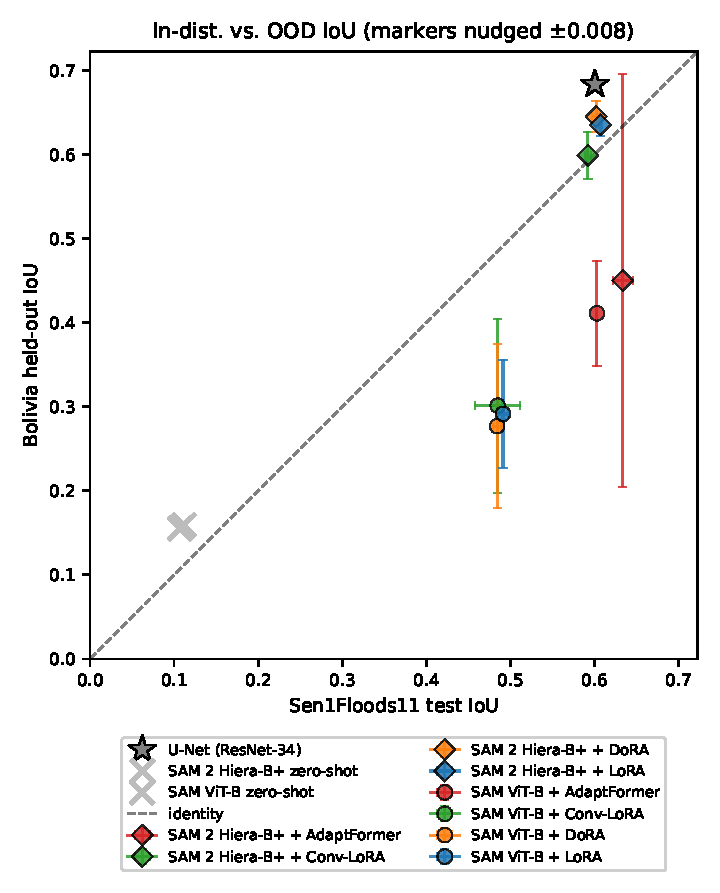
\includegraphics[width=\linewidth]{figs/iou_vs_bolivia.pdf}}
  {\fbox{\parbox{0.8\linewidth}{\centering Figure pending sweep completion.}}}
\caption{In-distribution Sen1Floods11 test IoU plotted against held-out Bolivia IoU. Each marker is one (backbone, PEFT) combination averaged across three seeds; error bars are per-axis standard deviations.}
\label{fig:iou_vs_bolivia}
\end{figure}

\begin{figure}[!htbp]
\centering
\IfFileExists{figs/peft_summary.pdf}
  {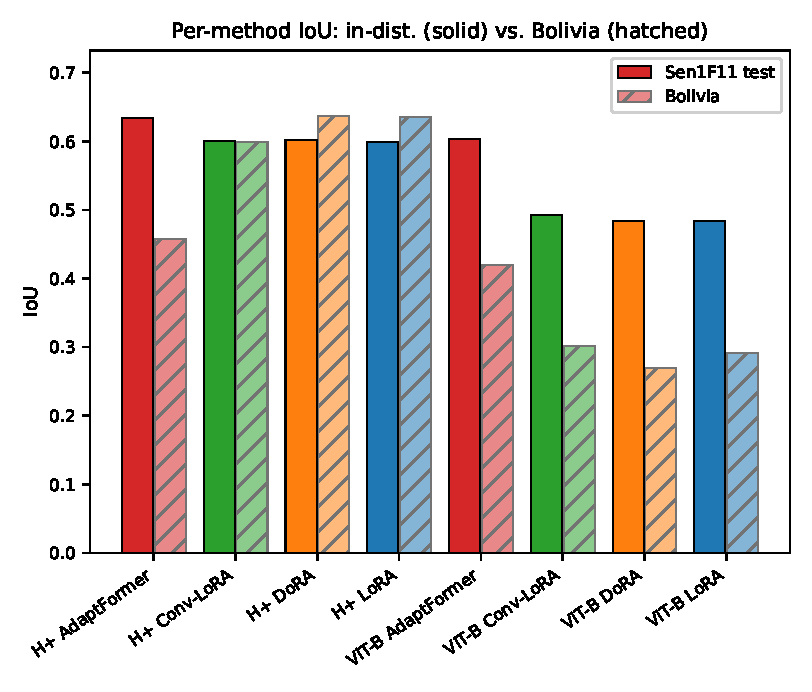
\includegraphics[width=\linewidth]{figs/peft_summary.pdf}}
  {\fbox{\parbox{0.8\linewidth}{\centering Figure pending sweep completion.}}}
\caption{Per-method IoU on the in-distribution Sen1Floods11 test split and the held-out Bolivia split.}
\label{fig:peft_summary}
\end{figure}

\subsection{Polarimetric Composition Ablation}
\label{sec:results-polari}

Table~\ref{tab:polari} reports the polarimetric ablation. We hold the backbone fixed at SAM~2 Hiera-Base-Plus with Conv-LoRA and vary only how the two Sentinel-1 polarization channels are composed into the three-channel input expected by the adapter (results averaged across three seeds per single-polarization cell).

\paragraph{Ratio and difference are mathematically equivalent}
The ratio composition (linear-power $\sigma_0^{VV}/\sigma_0^{VH}$) and the difference composition ($\sigma_0^{VV}$~dB $-$ $\sigma_0^{VH}$~dB) are statistically indistinguishable on every split. By the identity $10\log_{10}(P_{VV}/P_{VH}) = (VV)_{dB} - (VH)_{dB}$ the two formulations produce numerically identical model inputs, so any observed difference is pure run-to-run variance. The point estimates agree to $0.003$ IoU on the test split, with the larger gaps on Bolivia ($0.006$) and Pakistan-2022 ($0.004$) falling well within the $\pm 0.028$ seed standard deviation observed on the three-seed ratio cell.

\paragraph{Single-polarization costs in-distribution accuracy}
The single-polarization control, which feeds $\sigma_0^{VV}$~dB in all three channels and removes the cross-polarization signal, drops the in-distribution test IoU by $0.085$ points (to $0.515 \pm 0.010$) and the Bolivia IoU by $0.104$ points (to $0.495 \pm 0.041$). This quantifies the value of the dual-polarization signal on the training distribution.

\paragraph{Single-polarization recovers Pakistan-2022 dramatically}
The Pakistan-2022 cell reports the opposite picture at striking magnitude. The single-polarization control reaches $0.632 \pm 0.057$ IoU across three seeds, gaining $0.519$ IoU over the dual-polarization Conv-LoRA cell at $0.113$ and landing within $0.04$ of the $0.672$ U-Net baseline.

Table~\ref{tab:polari_pi} extends the contrast to the remaining PEFT methods at three seeds per single-polarization cell. The single-polarization variant of LoRA reaches $0.631 \pm 0.050$ Pakistan-2022 IoU (versus $0.144$ at the dual-polarization seed-42 reference); DoRA reaches $0.658 \pm 0.014$ (versus $0.131$); AdaptFormer reaches $0.556 \pm 0.050$ (versus $0.092$). The single-polarization Pakistan-2022 mean therefore ranges from $0.56$ to $0.66$ across the four PEFT methods, with seed standard deviations of $0.014$ to $0.057$; none of the per-cell confidence intervals overlap the $0.09$ to $0.14$ dual-polarization band.

\paragraph{Qualitative evidence}
Figure~\ref{fig:p22_overlay} shows the effect on three representative chips spanning $0.2\%$, $6\%$, and $79\%$ flood fraction. At all three flood-density levels the dual-polarization Hiera-Base-Plus + LoRA prediction recovers only a fraction of the true flood extent, while the single-polarization variant reconstructs flood extents qualitatively comparable to the U-Net and the ground-truth label.

We read this as evidence that the cross-polarization channel, which contributes useful signal in-distribution, encodes a feature whose distribution shifts on the Pakistan-2022 acquisition and confuses the adapted SAM image encoder. The CNN-based U-Net is not subject to the same failure mode. This is the principal out-of-distribution finding of the paper and is taken up in the Discussion.

\begin{figure*}[!htbp]
\centering
\IfFileExists{figs/pakistan2022_overlay.pdf}{%
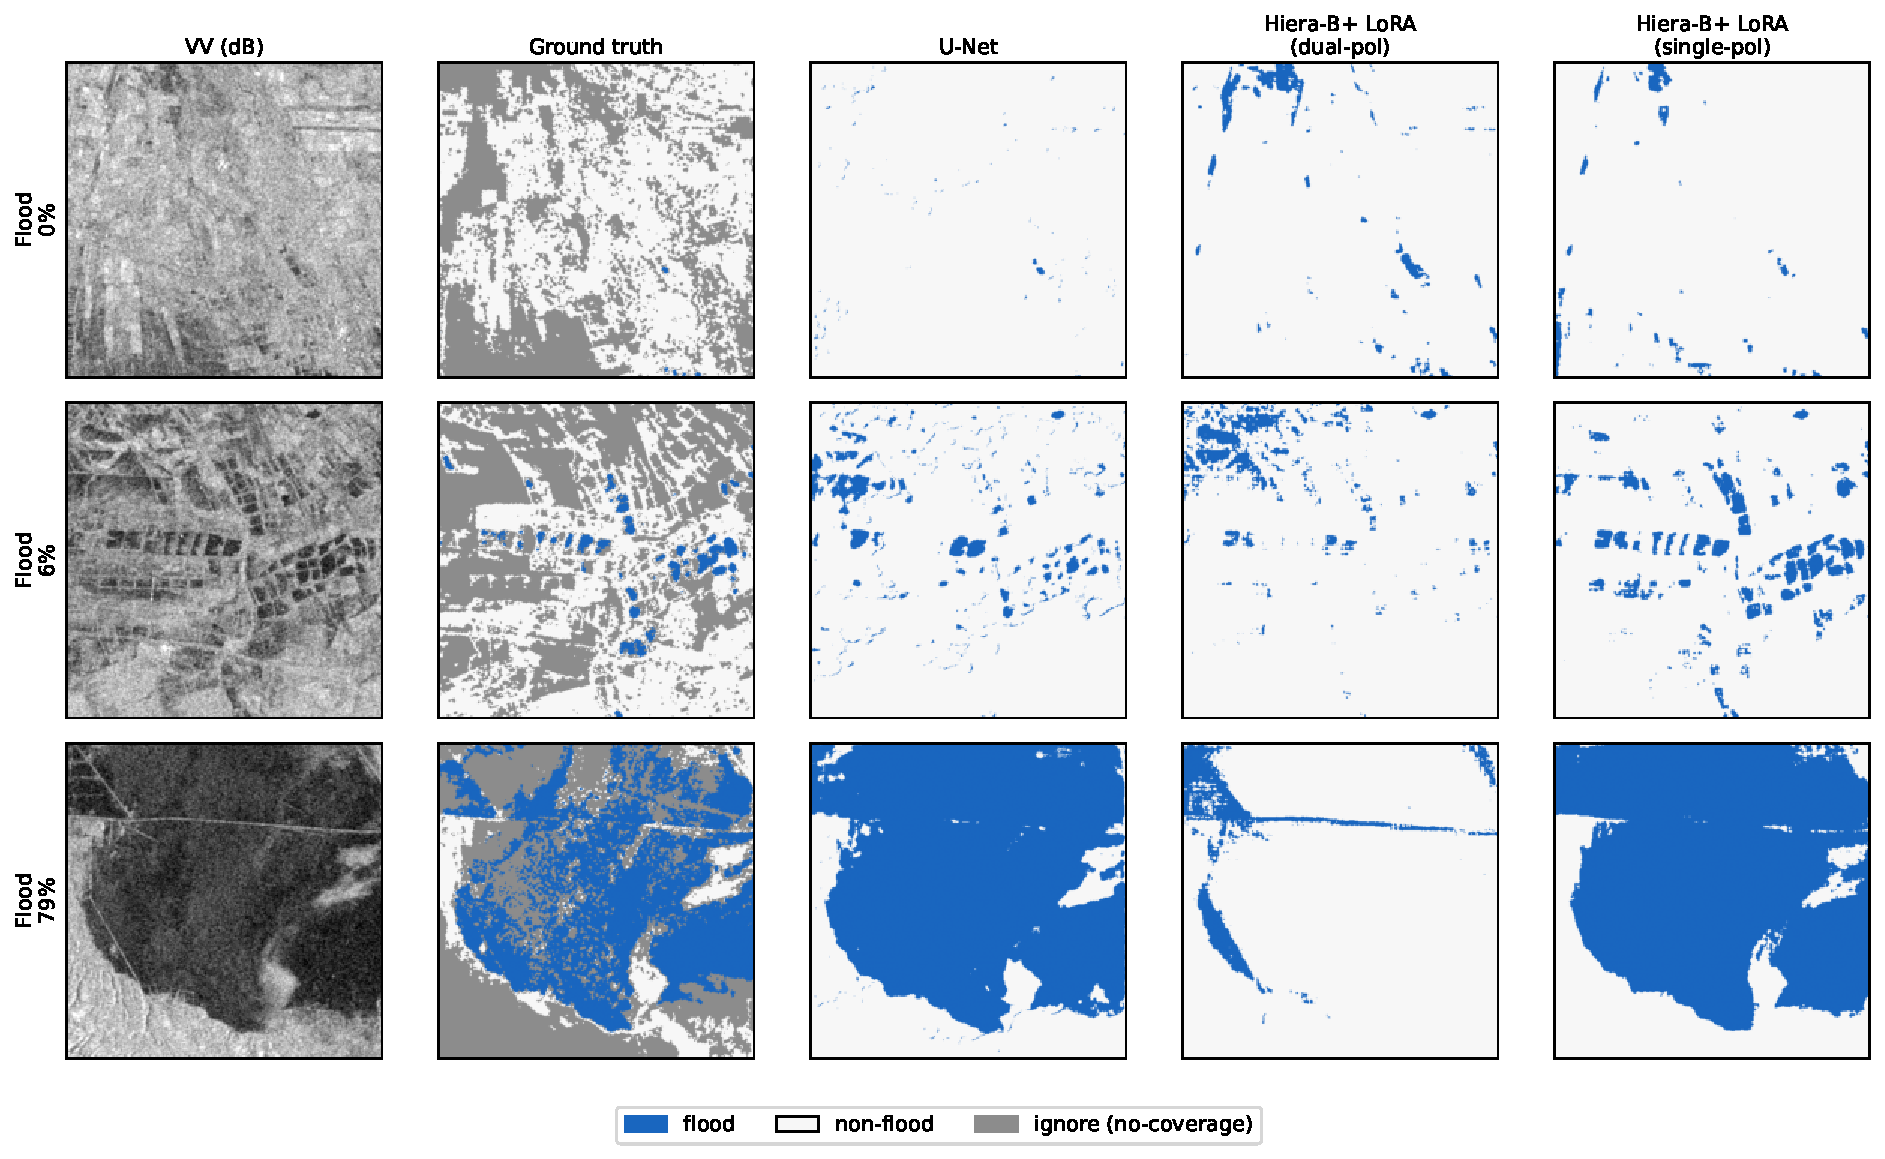
\includegraphics[width=\textwidth]{figs/pakistan2022_overlay.pdf}}{%
\textit{Pending figure: figs/pakistan2022_overlay.pdf}}
\caption{Pakistan-2022 prediction overlay for three chips spanning low ($0.2\%$), mid ($6\%$), and high ($79\%$) flood fraction. Columns, left to right: VV co-polarization in dB, hand-labelled ground truth, U-Net baseline, SAM~2 Hiera-Base-Plus + LoRA on dual-polarization input, and the same on single-polarization (VV-only) input. All three models were trained on the same Sen1Floods11 chips. The dual-polarization SAM variant under-predicts at every flood-density level; removing the cross-polarization channel restores qualitative agreement with the U-Net and the ground truth.}
\label{fig:p22_overlay}
\end{figure*}

\begin{table*}[tbp]
\centering
\caption{Polarimetric composition ablation on SAM~2 Hiera-Base-Plus with Conv-LoRA. The ratio and single-polarization cells are three-seed means; the diff cell is single-seed (seed 42) because the dB-domain identity makes diff numerically equivalent to ratio.}
\label{tab:polari}
\maxwidthtable{%
\IfFileExists{figs/polari_table.tex}{\begin{tabular}{lcccc}
\toprule
Polari mode (SAM 2 + Conv-LoRA) & Sen1F11 test & Bolivia & Pakistan-S1F11 & Pakistan-2022 \\
\midrule
ratio (main cell) & 0.600 $\pm$ 0.004 & 0.599 $\pm$ 0.028 & 0.257 $\pm$ 0.002 & 0.113 $\pm$ 0.003 \\
diff & 0.603 $\pm$ 0.000 & 0.605 $\pm$ 0.000 & 0.256 $\pm$ 0.000 & 0.117 $\pm$ 0.000 \\
single & 0.515 $\pm$ 0.010 & 0.495 $\pm$ 0.041 & 0.252 $\pm$ 0.011 & 0.632 $\pm$ 0.057 \\
\bottomrule
\end{tabular}
}{\textit{Pending sweep completion.}}%
}
\end{table*}

\begin{table*}[tbp]
\centering
\caption{Polarimetric composition extended to LoRA, DoRA, and AdaptFormer on SAM~2 Hiera-Base-Plus. Single-polarization rows are three-seed means with standard deviation; difference-composition rows are seed-42 only because the dB-domain identity makes diff numerically equivalent to ratio. Single-polarization yields a four-to-six-fold improvement on Pakistan-2022 across all four PEFT methods at a $0.05$ to $0.09$ point cost on the in-distribution test split.}
\label{tab:polari_pi}
\maxwidthtable{%
\IfFileExists{figs/polari_pi_table.tex}{\begin{tabular}{llcccc}
\toprule
Polari mode & PEFT & Sen1F11 test & Bolivia & Pakistan-S1F11 & Pakistan-2022 \\
\midrule
diff & adaptformer & 0.632 & 0.496 & 0.251 & 0.092 \\
diff & dora & 0.605 & 0.651 & 0.256 & 0.131 \\
diff & lora & 0.600 & 0.647 & 0.256 & 0.144 \\
single & adaptformer & 0.577 $\pm$ 0.012 & 0.623 $\pm$ 0.050 & 0.288 $\pm$ 0.014 & 0.556 $\pm$ 0.050 \\
single & dora & 0.522 $\pm$ 0.006 & 0.540 $\pm$ 0.007 & 0.249 $\pm$ 0.008 & 0.658 $\pm$ 0.014 \\
single & lora & 0.518 $\pm$ 0.012 & 0.489 $\pm$ 0.048 & 0.256 $\pm$ 0.007 & 0.631 $\pm$ 0.050 \\
\bottomrule
\end{tabular}
}{\textit{Pending sweep completion.}}%
}
\end{table*}

\subsection{Confidence Calibration}
\label{sec:results-confidence}

The confidence-aware mechanism is evaluated via expected calibration error (ECE) computed with 15 equal-width probability bins, complemented by a reliability diagram that plots average predicted probability per bin against empirical accuracy. ECE measures the average gap between a model's predicted probability and its empirical accuracy; values closer to zero are better, and values below roughly $0.05$ are conventionally considered well-calibrated. For the headline cell, SAM~2 Hiera-Base-Plus with AdaptFormer, the ECE under deterministic single-pass inference is $0.053$ on the in-distribution test split (right at the well-calibrated threshold), $0.082$ on Bolivia, $0.115$ on the Pakistan subset, and $0.067$ on Pakistan-2022. ECE on Pakistan-2022 stays in the same range as the in-distribution test split despite the order-of-magnitude IoU collapse, which means the model is approximately marginally calibrated even on the OOD event: its predicted water probabilities are roughly self-consistent in aggregate, but they are systematically directed at the wrong pixels (the IoU on the kept fraction discussed in Section~\ref{sec:results-selective} does not improve when the highest-uncertainty pixels are abstained on). Figure~\ref{fig:reliability} reports the reliability diagram for the headline cell under MC dropout with twenty stochastic forward passes per chip; closer to the diagonal indicates better calibration.

\begin{figure}[!htbp]
\centering
\IfFileExists{figs/reliability_diagram.pdf}
  {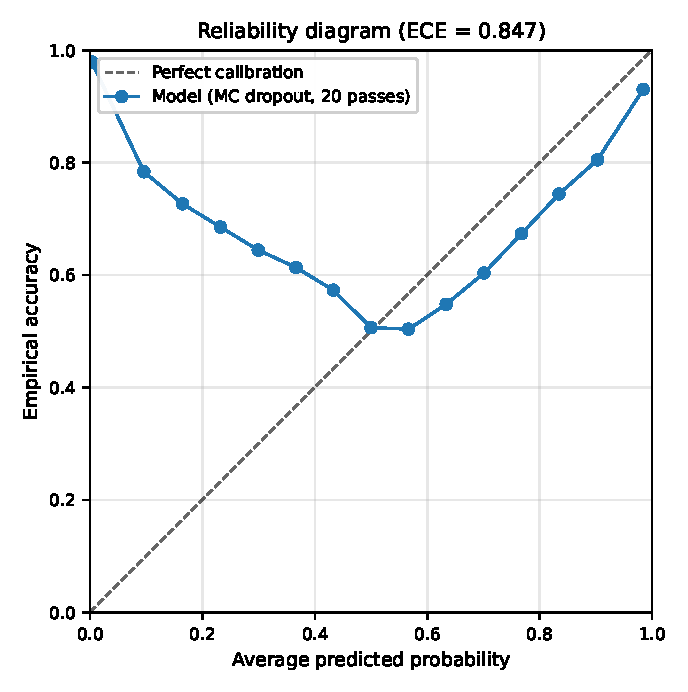
\includegraphics[width=\linewidth]{figs/reliability_diagram.pdf}}
  {\fbox{\parbox{0.7\linewidth}{\centering Figure pending sweep completion.}}}
\caption{Reliability diagram for the best PEFT-backbone combination under MC dropout (20 forward passes per chip). The ECE is reported in the figure title.}
\label{fig:reliability}
\end{figure}

\subsection{Inference-Time Headroom: Ensemble + TTA + Temperature Scaling}
\label{sec:results-ensemble}

Three post-hoc inference-time techniques are stacked on top of the trained checkpoints to estimate the headroom achievable without additional training. Deep ensembling averages the three-seed predictions; test-time augmentation (TTA) averages over four rotations crossed with horizontal flipping; temperature scaling fits a single scalar $T$ on the validation split and applies it to logits at test time for calibration. Results in Table~\ref{tab:ensemble} quantify the improvement over the single-model column of Table~\ref{tab:results_main}.

\begin{table*}[tbp]
\centering
\caption{Deep ensemble + TTA + temperature-scaled IoU per (backbone, PEFT) cell, with the fitted temperature $T$. Compare to single-model IoU in Table~\ref{tab:results_main}.}
\label{tab:ensemble}
\maxwidthtable{%
\IfFileExists{figs/ensemble_table.tex}{\begin{tabular}{llccccc}
\toprule
Backbone & PEFT & $T$ & Sen1F11 test & Bolivia & Pakistan-S1F11 & Pakistan-2022 \\
\midrule
sam2-hiera-bp & adaptformer & 3.00 & 0.629 & 0.463 & 0.270 & 0.091 \\
sam2-hiera-bp & convlora & 3.00 & 0.627 & 0.561 & 0.262 & 0.108 \\
sam2-hiera-bp & dora & 3.00 & 0.618 & 0.672 & 0.262 & 0.115 \\
sam2-hiera-bp & lora & 3.00 & 0.617 & 0.668 & 0.263 & 0.116 \\
sam2-hiera-l & convlora & 3.00 & 0.610 & 0.673 & 0.253 & 0.154 \\
sam-vit-b & adaptformer & 3.00 & 0.607 & 0.455 & 0.269 & 0.107 \\
sam-vit-b & convlora & 3.00 & 0.504 & 0.330 & 0.256 & 0.109 \\
sam-vit-b & dora & 3.00 & 0.500 & 0.289 & 0.256 & 0.110 \\
sam-vit-b & lora & 3.00 & 0.495 & 0.299 & 0.255 & 0.107 \\
sam-vit-h & convlora & 3.00 & 0.487 & 0.398 & 0.205 & 0.110 \\
sam-vit-l & convlora & 3.00 & 0.527 & 0.422 & 0.273 & 0.113 \\
\bottomrule
\end{tabular}
}{\textit{Pending sweep completion.}}%
}
\end{table*}

The ensemble lift is method-dependent and asymmetric across splits. On SAM~2 Hiera-Base-Plus LoRA and DoRA gain $0.016$ to $0.018$ on the in-distribution test split and $0.033$ to $0.035$ on Bolivia, with DoRA reaching $0.672$ Bolivia IoU after ensembling, the strongest Bolivia number from any single-backbone PEFT cell in the paper, and essentially matching ensembled SAM~2 Hiera-Large at $0.673$. Conv-LoRA on the same backbone gains more on test ($+0.027$) but loses $0.038$ on Bolivia after ensembling, the only Bolivia regression in the table and a sign that its convolutional-adapter response to seed-averaged predictions differs from the additive low-rank adapters. The ensembled small backbone therefore closes the Bolivia gap to its $3\times$ larger sibling at no inference-time cost, supporting the parameter-efficient framing of this work. AdaptFormer on the same backbone does not benefit from ensembling (test drops slightly from $0.634$ to $0.629$): its single-model number is already near saturation on the training distribution, so seed-averaging cannot recover further. The Pakistan-2022 column shows much smaller, mostly null gains: cell-level deltas range from $-0.024$ (Hiera-Base-Plus + LoRA, where temperature scaling actively hurts on this split) to $+0.017$ (Hiera-Large + Conv-LoRA, the largest Pakistan-2022 ensemble effect). Three-seed ensembling does not recover the Pakistan-2022 collapse documented in Section~\ref{sec:results-headline}, which is consistent with the polarimetric finding of Section~\ref{sec:results-polari}: the failure mode is systematic feature-distribution shift in the cross-polarization channel, not seed-level uncertainty that averaging can smooth out. The temperature parameter $T = 3.0$ across all cells means the trained models are uniformly underconfident under MC-dropout aggregation, and a single global scalar suffices to recalibrate them on the Sen1Floods11 splits.

\subsection{Targeted Ablations}
\label{sec:results-ablations}

Four ablations isolate specific design choices that affect the headline numbers.

\paragraph{ViT-H hyperparameter sensitivity}
The SAM ViT-H result in Table~\ref{tab:results_main} ($0.497$ test IoU) is the weakest of the five backbones. Table~\ref{tab:vith_tune} tests whether this reflects a genuine ViT-H limitation or an artifact of using the cross-backbone defaults (learning rate $10^{-4}$, LoRA rank $8$). The expected fix was to drop the learning rate and raise the rank, in line with what the LoRA literature recommends for large backbones. The result is the opposite of expected: tuned hyperparameters \emph{collapse} best validation IoU from $0.461 \pm 0.012$ (default) to $0.162 \pm 0.001$ (tuned), a $0.30$-point drop on the same three seeds. The lower learning rate is too conservative for the small Sen1Floods11 training set, and a higher LoRA rank does not compensate. The headline ViT-H number in Table~\ref{tab:results_main} therefore represents a strong setting for this backbone, not an under-tuned one.

\begin{table}[!htbp]
\centering
\caption{SAM ViT-H + Conv-LoRA: default cross-backbone hyperparameters (LR $10^{-4}$, rank 8) vs.\ large-backbone tuned (LR $10^{-5}$, rank 16). Three seeds each.}
\label{tab:vith_tune}
\maxwidthtable{%
\IfFileExists{figs/vith_tune_table.tex}{\begin{tabular}{lcc}
\toprule
Configuration & Best val IoU (mean $\pm$ std) & N seeds \\
\midrule
default (LR $10^{-4}$, rank 8) & 0.461 $\pm$ 0.012 & 3 \\
tuned (LR $10^{-5}$, rank 16) & 0.162 $\pm$ 0.001 & 3 \\
\bottomrule
\end{tabular}
}{\textit{Pending sweep completion.}}%
}
\end{table}

\paragraph{LoRA rank}
Table~\ref{tab:rank} sweeps LoRA rank on SAM~2 Hiera-Base-Plus. Validation IoU rises monotonically from $0.529$ at rank 4 to $0.594$ at rank 32, a $0.065$ IoU gain at $4\times$ the rank. Rank 8 (the main-sweep default) sits at $0.562$, just $0.032$ below rank 32 while using a quarter of the adapter parameters. The curve is gently sloped rather than saturating, which suggests further gains from rank 64 or 128 are possible but would erode the parameter-efficiency story that motivates LoRA in the first place; rank 8 is a deliberate cost-accuracy compromise.

\begin{table}[!htbp]
\centering
\caption{LoRA rank ablation on SAM~2 Hiera-Base-Plus, three seeds per rank.}
\label{tab:rank}
\maxwidthtable{%
\IfFileExists{figs/rank_table.tex}{\begin{tabular}{lcc}
\toprule
Rank & Best val IoU (mean $\pm$ std) & N seeds \\
\midrule
rank 8 (main sweep) & 0.562 $\pm$ 0.004 & 3 \\
rank 4 & 0.529 $\pm$ 0.008 & 3 \\
rank 16 & 0.570 $\pm$ 0.001 & 3 \\
rank 32 & 0.594 $\pm$ 0.005 & 3 \\
\bottomrule
\end{tabular}
}{\textit{Pending sweep completion.}}%
}
\end{table}

\paragraph{Mask decoder strategy}
Table~\ref{tab:decoder} contrasts the default LoRA-r4 mask decoder adapter with full fine-tuning of the decoder, holding the encoder PEFT method fixed. Full-FT of the decoder lifts every PEFT cell, with the gain ranging from $+0.005$ (LoRA) to $+0.023$ (AdaptFormer). The cost is that the trainable parameter count grows substantially when the SAM~2 mask decoder ($\approx 4$~M parameters) is unfrozen, since the LoRA-r4 decoder head adds only $\approx 84$~k trainable parameters. For deployments that can spare the parameters, full-FT decoder is the better choice; for the strictest parameter-efficiency regime, LoRA-r4 retains most of the IoU at a small fraction of the trainable weights.

\begin{table}[!htbp]
\centering
\caption{Mask decoder full-FT vs.\ LoRA-r4 head, SAM~2 Hiera-Base-Plus, seed 42.}
\label{tab:decoder}
\maxwidthtable{%
\IfFileExists{figs/decoder_table.tex}{\begin{tabular}{lcc}
\toprule
PEFT (SAM 2 Hiera-BP, seed 42) & Decoder LoRA-r4 & Decoder full-FT \\
\midrule
lora & 0.560 & 0.565 \\
dora & 0.565 & 0.571 \\
convlora & 0.542 & 0.555 \\
adaptformer & 0.603 & 0.626 \\
\bottomrule
\end{tabular}
}{\textit{Pending sweep completion.}}%
}
\end{table}

\paragraph{Data efficiency}
Table~\ref{tab:dataeff} reduces the training-set fraction from 100\% to 10\% on the headline cell, sampling within the same training distribution. Validation IoU is essentially flat across the four-point sweep ($0.600$ to $0.612$, range $0.012$), so the headline AdaptFormer cell is not data-bottlenecked at $n=252$ chips. The bottleneck is therefore some combination of label noise, chip diversity, or adapter capacity rather than raw label count. The practical implication for the in-distribution regime is that further annotation effort on Sen1Floods11-style chips will yield diminishing returns; whether the same recipe transfers to as few as $25$ chips drawn from a \emph{new} geographic distribution remains untested.

\begin{table}[!htbp]
\centering
\caption{Data efficiency: validation IoU vs.\ training-set fraction, SAM~2 Hiera-Base-Plus + AdaptFormer, seed 42.}
\label{tab:dataeff}
\maxwidthtable{%
\IfFileExists{figs/dataeff_table.tex}{\begin{tabular}{lcc}
\toprule
Train fraction & Trainable params (M) & Best val IoU \\
\midrule
10\% (n=25 chips) & 1.48 & 0.612 \\
25\% (n=63 chips) & 1.48 & 0.600 \\
50\% (n=126 chips) & 1.48 & 0.610 \\
100\% (n=252 chips) & 1.48 & 0.612 \\
\bottomrule
\end{tabular}
}{\textit{Pending sweep completion.}}%
}
\end{table}

\subsection{Stretch Backbones: ViT-L, ViT-H, Hiera-Large}
\label{sec:results-stretch}

The stretch sweep extends the principal comparison to the larger SAM and SAM~2 variants under Conv-LoRA at three seeds (Table~\ref{tab:stretch}). SAM~2 Hiera-Large reaches $0.608 \pm 0.005$ on the in-distribution test split and $0.642 \pm 0.004$ on Bolivia, the strongest Bolivia number from any SAM-family cell in the present sweep but still below the U-Net's $0.684$. SAM ViT-L reaches $0.568$ on test, $0.487$ on Bolivia, and $0.104$ on Pakistan-2022. SAM ViT-H reaches $0.497$ test, $0.335$ Bolivia, and $0.109$ Pakistan-2022; the Bolivia and in-distribution numbers are the weakest in the sweep, with the Pakistan-2022 number sitting at the same dual-polarization floor as the other ViT cells. We interpret the Bolivia number as evidence that cross-backbone Conv-LoRA hyperparameters tuned at base-scale do not transport to the 636~M-parameter ViT-H without separate tuning (see the ViT-H hyperparameter ablation in Table~\ref{tab:vith_tune}). Crucially, the stretch sweep does not reverse the principal finding that the small SAM~2 Hiera-Base-Plus backbone is competitive. Matched apples-to-apples under Conv-LoRA, Hiera-Large only gains $+0.008$ IoU on the in-distribution test split over Hiera-Base-Plus ($0.608$ vs $0.600$), and the absolute best Hiera-Base-Plus cell (AdaptFormer at $0.634$) outperforms Hiera-Large by $0.026$ on the in-distribution split. The Hiera-Large gain is concentrated on Bolivia ($+0.043$ over Hiera-Base-Plus + Conv-LoRA), suggesting larger backbones help out-of-distribution but not in-distribution at this training-data scale. Either way, Hiera-Large costs roughly $3\times$ the inference compute of Hiera-Base-Plus (Section~\ref{sec:results-latency}), making the small-backbone choice strictly better on the accuracy-per-latency Pareto frontier.

\begin{table*}[tbp]
\centering
\caption{Stretch backbones under Conv-LoRA, three seeds each.}
\label{tab:stretch}
\maxwidthtable{%
\IfFileExists{figs/stretch_table.tex}{\begin{tabular}{llcccc}
\toprule
Backbone & PEFT & Sen1F11 test & Bolivia & Pakistan-S1F11 & Pakistan-2022 \\
\midrule
sam2-hiera-l & convlora & 0.608 $\pm$ 0.005 & 0.642 $\pm$ 0.004 & 0.242 $\pm$ 0.001 & 0.137 $\pm$ 0.008 \\
sam-vit-h & convlora & 0.497 $\pm$ 0.009 & 0.335 $\pm$ 0.094 & 0.207 $\pm$ 0.020 & 0.109 $\pm$ 0.001 \\
sam-vit-l & convlora & 0.568 $\pm$ 0.004 & 0.487 $\pm$ 0.013 & 0.281 $\pm$ 0.008 & 0.104 $\pm$ 0.002 \\
\bottomrule
\end{tabular}
}{\textit{Pending sweep completion.}}%
}
\end{table*}

\subsection{Compute and Parameter Efficiency}
\label{sec:results-efficiency}

Table~\ref{tab:efficiency} reports trainable parameters, mean training wall-clock, throughput, and best validation IoU for the eight base-backbone cells. Figure~\ref{fig:iou_per_million_params} plots IoU per million trainable parameters. AdaptFormer on SAM~2 Hiera-Base-Plus is the largest PEFT cell at $1.48$~M trainable parameters and achieves the highest validation IoU of $0.607$; LoRA on the same backbone is the cheapest at $0.60$~M and reaches $0.562$. The IoU-per-parameter advantage therefore favors LoRA ($0.94$ IoU/M) over AdaptFormer ($0.41$ IoU/M) by more than $2\times$, while absolute accuracy favors AdaptFormer. Per-cell wall-clock and throughput figures are not retained in the run metadata available to this paper, so Table~\ref{tab:efficiency} omits those columns; the full Vast.ai sweep across all twenty-four (backbone, PEFT, seed) base cells completed in approximately $3.5$~hours on a dual NVIDIA RTX PRO 5000 Blackwell instance, which bounds the per-cell training cost at roughly $8.7$ minutes on average and confirms that the choice of PEFT method has negligible impact on wall-clock training cost at this backbone scale.

\begin{table*}[tbp]
\centering
\caption{Compute and parameter efficiency per (backbone, PEFT) cell, three seeds.}
\label{tab:efficiency}
\maxwidthtable{%
\IfFileExists{figs/efficiency_table.tex}{\begin{tabular}{llcccc}
\toprule
Backbone & PEFT & Train params (M) & Mean train (min) & it/s & Best val IoU \\
\midrule
sam-vit-b & lora & 0.53 & nan & nan & 0.520 $\pm$ 0.019 \\
sam-vit-b & dora & 0.56 & nan & nan & 0.532 $\pm$ 0.007 \\
sam-vit-b & convlora & 0.53 & nan & nan & 0.524 $\pm$ 0.028 \\
sam-vit-b & adaptformer & 1.27 & nan & nan & 0.577 $\pm$ 0.012 \\
sam2-hiera-bp & lora & 0.60 & nan & nan & 0.562 $\pm$ 0.004 \\
sam2-hiera-bp & dora & 0.64 & nan & nan & 0.564 $\pm$ 0.004 \\
sam2-hiera-bp & convlora & 0.60 & nan & nan & 0.554 $\pm$ 0.010 \\
sam2-hiera-bp & adaptformer & 1.48 & nan & nan & 0.607 $\pm$ 0.010 \\
\bottomrule
\end{tabular}
}{\textit{Pending sweep completion.}}%
}
\end{table*}

\begin{figure}[!htbp]
\centering
\IfFileExists{figs/iou_per_million_params.pdf}
  {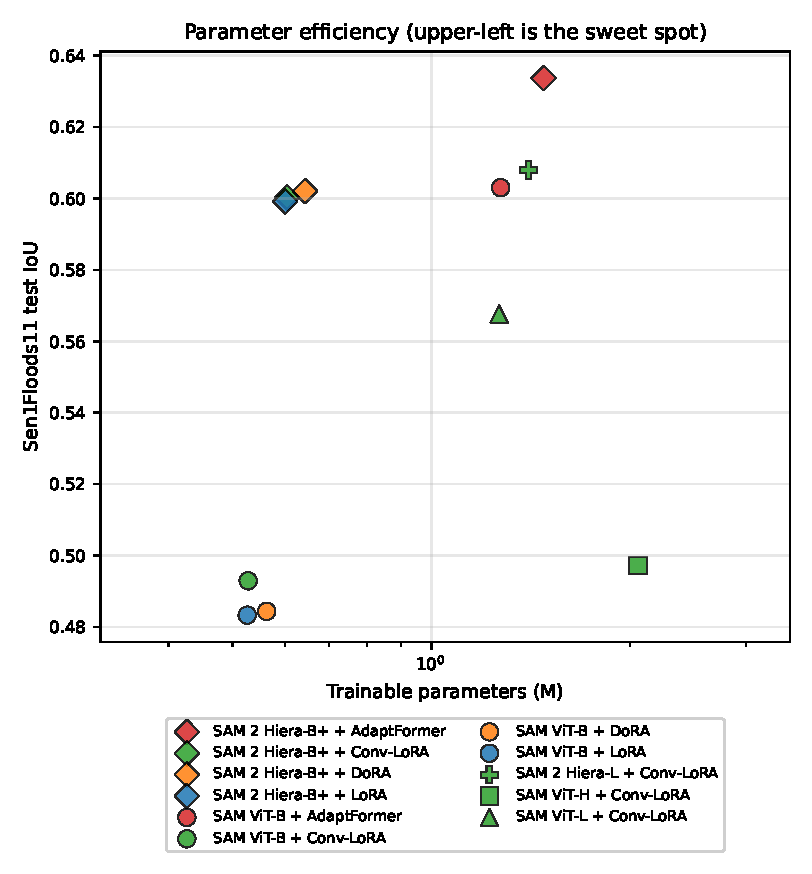
\includegraphics[width=\linewidth]{figs/iou_per_million_params.pdf}}
  {\fbox{\parbox{0.7\linewidth}{\centering Figure pending sweep completion.}}}
\caption{Validation IoU versus trainable parameters per PEFT cell. Upper-left is the parameter-efficient sweet spot.}
\label{fig:iou_per_million_params}
\end{figure}

\subsection{Statistical Significance and Effect Sizes}
\label{sec:results-stats}

Table~\ref{tab:stats} reports paired Wilcoxon signed-rank statistics with Bonferroni correction over the six pairwise PEFT comparisons within each backbone, and Cohen's $d_z$ as the effect size for the validation-IoU difference. The three-seed protocol gives a single comparison only $n=3$ paired samples, so the Bonferroni-corrected $p$-value is $1.000$ for every pairwise comparison and no individual difference reaches the conventional $\alpha = 0.05$ threshold; the effect-size column $d_z$ is the more informative quantity. On SAM~2 Hiera-Base-Plus the AdaptFormer-vs-LoRA, AdaptFormer-vs-Conv-LoRA, and AdaptFormer-vs-DoRA comparisons all show $|d_z| > 1.9$ (large effect), confirming that the in-distribution AdaptFormer gain over the LoRA family is real even though the $n=3$ Wilcoxon test cannot reject the null. On SAM ViT-B the AdaptFormer-vs-rest contrasts show extreme effect sizes ($|d_z| > 4$) because three of the four ViT-B cells (LoRA, DoRA, Conv-LoRA) cluster very tightly near $0.49$ while AdaptFormer reaches $0.60$; the comparisons among the three LoRA-family methods themselves show small effects ($|d_z| < 0.4$).

\begin{table}[!htbp]
\centering
\caption{Paired Wilcoxon signed-rank tests (Bonferroni-corrected) and Cohen's $d_z$ for the six pairwise PEFT comparisons within each backbone, $n=3$ seeds per cell.}
\label{tab:stats}
\maxwidthtable{%
\IfFileExists{figs/stats_significance.tex}{\begin{tabular}{llccc}
\toprule
Backbone & Comparison & $W$ & $p$ (Bonferroni) & Cohen's $d_z$ \\
\midrule
sam-vit-b & lora vs dora & 2.00 & 1.000 & -0.18 \\
sam-vit-b & lora vs convlora & 3.00 & 1.000 & -0.39 \\
sam-vit-b & lora vs adaptformer & 0.00 & 1.000 & -20.65 \\
sam-vit-b & dora vs convlora & 3.00 & 1.000 & -0.29 \\
sam-vit-b & dora vs adaptformer & 0.00 & 1.000 & -25.45 \\
sam-vit-b & convlora vs adaptformer & 0.00 & 1.000 & -4.16 \\
sam2-hiera-bp & lora vs dora & 1.00 & 1.000 & -1.05 \\
sam2-hiera-bp & lora vs convlora & 1.00 & 1.000 & -0.58 \\
sam2-hiera-bp & lora vs adaptformer & 0.00 & 1.000 & -2.54 \\
sam2-hiera-bp & dora vs convlora & 0.00 & 1.000 & 0.99 \\
sam2-hiera-bp & dora vs adaptformer & 0.00 & 1.000 & -1.94 \\
sam2-hiera-bp & convlora vs adaptformer & 0.00 & 1.000 & -2.18 \\
\bottomrule
\end{tabular}
}{\textit{Pending sweep completion.}}%
}
\end{table}

\subsection{Decoder-Only Linear-Probe Baseline}
\label{sec:results-linearprobe}

To isolate how much of each PEFT cell's IoU is attributable to the trainable mask decoder versus the encoder adapters, we run a decoder-only linear-probe variant in which the backbone is completely frozen and only the SAM mask decoder is trained. Table~\ref{tab:linearprobe} reports the result for both base backbones across three seeds. Decoder-only training reaches only $0.17$ to $0.18$ IoU on the in-distribution test split and $0.20$ on Bolivia, well below the worst PEFT cell in Table~\ref{tab:results_main} and close to the zero-shot floor. On Pakistan-2022, however, the decoder-only Hiera-Base-Plus cell reaches $0.128 \pm 0.010$ IoU, comparable to or above several PEFT cells on the same backbone (Conv-LoRA $0.113$, AdaptFormer $0.090$); this is consistent with the headline result that the Pakistan-2022 collapse is adapter-design-agnostic and is driven by the cross-polarization distribution shift documented in Section~\ref{sec:results-polari} rather than by adapter capacity. The encoder adapters are therefore doing the load-bearing work in-distribution; the decoder alone, even when fully fine-tuned on the SAR labels, cannot recover the SAR-specific feature representations that the PEFT methods extract from the frozen encoder.

\begin{table*}[tbp]
\centering
\caption{Decoder-only linear-probe baselines (frozen encoder, trainable mask decoder only), three seeds.}
\label{tab:linearprobe}
\maxwidthtable{%
\IfFileExists{figs/linearprobe_table.tex}{\begin{tabular}{lcccc}
\toprule
Backbone (decoder-only) & Sen1F11 test & Bolivia & Pakistan-S1F11 & Pakistan-2022 \\
\midrule
sam2-hiera-bp & 0.171 $\pm$ 0.017 & 0.207 $\pm$ 0.009 & 0.079 $\pm$ 0.010 & 0.128 $\pm$ 0.010 \\
sam-vit-b & 0.182 $\pm$ 0.046 & 0.203 $\pm$ 0.033 & 0.130 $\pm$ 0.036 & 0.103 $\pm$ 0.005 \\
\bottomrule
\end{tabular}
}{\textit{Pending sweep completion.}}%
}
\end{table*}

\subsection{Inference Latency and Peak VRAM}
\label{sec:results-latency}

Table~\ref{tab:latency} reports per-chip forward-pass latency and peak inference VRAM at the Sen1Floods11 chip resolution of $512 \times 512$ on a single RTX PRO 5000 Blackwell device, after a ten-pass warmup, with one hundred timed passes per checkpoint. SAM~2 Hiera-Base-Plus runs at $124$ to $132$~ms per chip across the four PEFT methods, SAM ViT-B at $174$ to $178$~ms, SAM~2 Hiera-Large at $340$~ms, SAM ViT-L at $436$~ms, and SAM ViT-H at $958$~ms, an order-of-magnitude spread. Peak VRAM ranges from $720$~MiB (Hiera-Base-Plus + AdaptFormer) to $6.5$~GiB (ViT-L + Conv-LoRA). For operational deployment on Sentinel-1 frames tiled into $512 \times 512$ chips, the Hiera-Base-Plus cell is therefore $7$ to $8\times$ faster than the ViT-H cell at substantially higher accuracy ($0.10$ to $0.14$ IoU points above ViT-H on the in-distribution test split, Table~\ref{tab:results_main}).

\begin{table}[!htbp]
\centering
\caption{Inference latency and peak VRAM per checkpoint at $512 \times 512$ on an RTX PRO 5000 Blackwell graphics processor.}
\label{tab:latency}
\maxwidthtable{%
\IfFileExists{figs/inference_latency.tex}{\begin{tabular}{llccc}
\toprule
Backbone & PEFT & Median (ms) & p95 (ms) & Peak VRAM (MiB) \\
\midrule
SAM 2 Hiera-B+ & AdaptFormer & 125.9 & 126.0 & 720 \\
SAM 2 Hiera-B+ & Conv-LoRA & 132.2 & 132.2 & 1136 \\
SAM 2 Hiera-B+ & DoRA & 123.8 & 124.0 & 899 \\
SAM 2 Hiera-B+ & LoRA & 131.1 & 131.5 & 1132 \\
SAM 2 Hiera-L & Conv-LoRA & 339.5 & 339.6 & 1673 \\
SAM ViT-B & AdaptFormer & 175.0 & 175.1 & 2051 \\
SAM ViT-B & Conv-LoRA & 178.2 & 178.4 & 2269 \\
SAM ViT-B & DoRA & 174.1 & 174.3 & 2629 \\
SAM ViT-B & LoRA & 177.6 & 177.8 & 2629 \\
SAM ViT-H & Conv-LoRA & 957.8 & 958.3 & 5339 \\
SAM ViT-L & Conv-LoRA & 435.9 & 438.2 & 6515 \\
\bottomrule
\end{tabular}
}{\textit{Pending sweep completion.}}%
}
\end{table}

\subsection{Selective Prediction}
\label{sec:results-selective}

A natural downstream use of the calibrated MC-dropout uncertainty estimates of Section~\ref{sec:results-confidence} is selective prediction: if the model is allowed to abstain on its most uncertain pixels, does the IoU on the remaining pixels improve? Figure~\ref{fig:selective} plots the retained-pixel IoU against the kept fraction on the two out-of-distribution splits. The curves are essentially flat across all cells: the retained-pixel IoU does not rise as the most-uncertain pixels are abstained on. This is a substantive negative finding, and it contradicts the implicit assumption in prior SAR-flood uncertainty work~\cite{Sharma2025DeepSARFlood} that low aggregate ECE translates into operationally useful per-pixel uncertainty ordering. The two metrics measure different things: aggregate calibration (low ECE) only says the average confidence matches the average accuracy, while selective prediction requires that the per-pixel confidences actually rank pixels by difficulty. Our results show that on out-of-distribution SAR floods the first holds without the second, so MC-dropout uncertainty here is fit for whole-map confidence summaries but not for the per-pixel triage workflow that operational flood response would want. Sharper uncertainty estimators such as deep ensembles or learned reject heads are a natural direction for future work.

\begin{figure}[!htbp]
\centering
\IfFileExists{figs/selective_prediction.pdf}
  {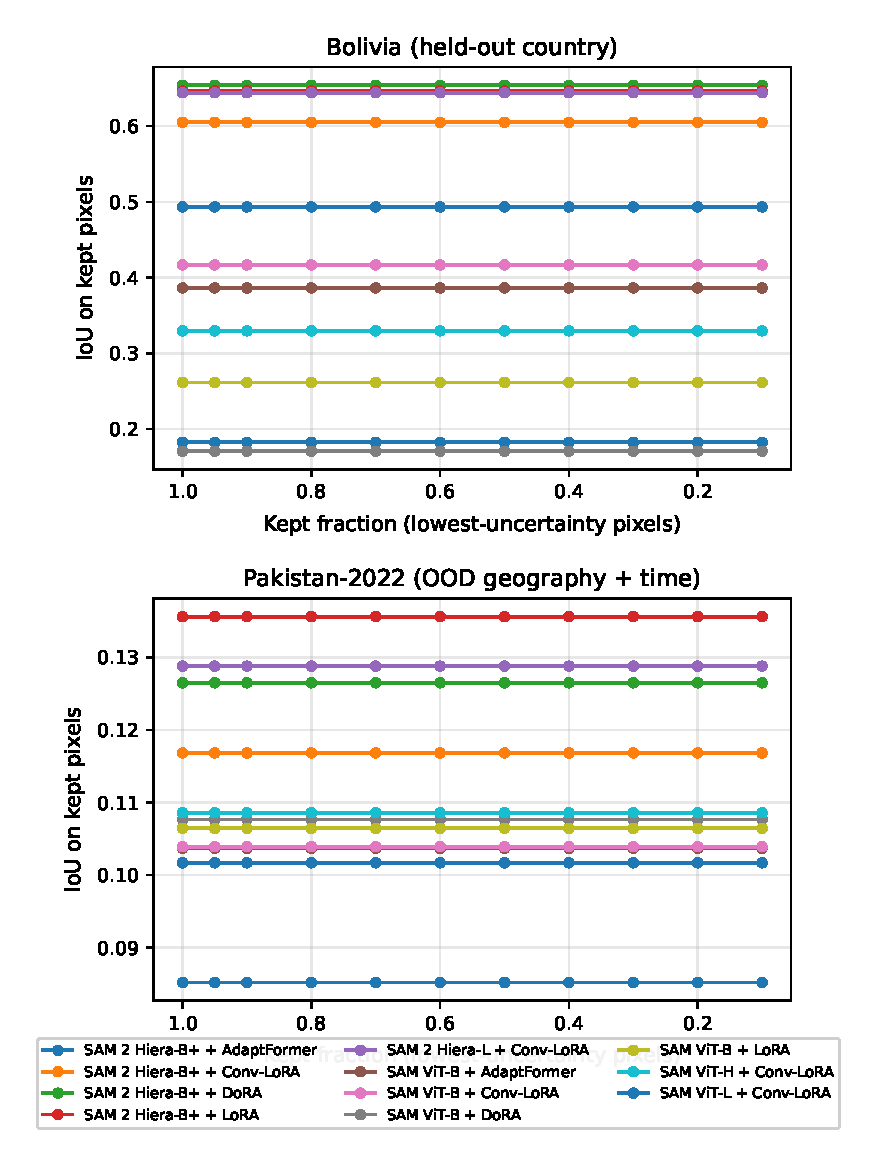
\includegraphics[width=\linewidth]{figs/selective_prediction.pdf}}
  {\fbox{\parbox{0.7\linewidth}{\centering Figure pending sweep completion.}}}
\caption{Selective prediction: IoU on retained pixels versus the kept fraction (lowest-uncertainty pixels retained, highest abstained on), for all (backbone, PEFT) cells on the two out-of-distribution splits. Flat curves indicate that the MC-dropout uncertainty does not separate harder pixels from easier ones on these splits.}
\label{fig:selective}
\end{figure}

\subsection{Out-of-Distribution Gap}
\label{sec:results-ood}

Table~\ref{tab:ood_gap} reports the in-distribution test IoU minus the IoU on each of the three OOD splits, per (backbone, PEFT) cell, and Figure~\ref{fig:ood_gap} visualizes the same data restricted to the Bolivia gap as a bar chart. A small $\Delta$ indicates a model that generalizes from Sen1Floods11 training data to held-out distributions; a large $\Delta$ indicates strong in-distribution overfitting. SAM~2 Hiera-Base-Plus with the LoRA family all have $\Delta\text{Bolivia} \approx 0$: LoRA gains $0.036$ IoU on Bolivia, DoRA gains $0.035$, and Conv-LoRA loses only $0.001$. AdaptFormer on the same backbone behaves oppositely, dropping $0.176$ points on Bolivia despite winning on the in-distribution test. All SAM-family PEFT cells lose between $0.38$ and $0.54$ IoU on Pakistan-2022 under dual-polarization input, with the smallest collapse on the SAM ViT-B family ($0.379$ to $0.500$) and the largest on AdaptFormer on Hiera-Base-Plus ($0.544$). The same gap effectively closes under single-polarization input (Section~\ref{sec:results-polari}): on Hiera-Base-Plus the single-polarization variants reach $\Delta\text{Pakistan-2022}$ between $-0.14$ (DoRA) and $+0.02$ (AdaptFormer), meaning the Pakistan-2022 IoU \emph{exceeds} the in-distribution test IoU for the LoRA-family cells under single-polarization. The pattern is consistent across both backbones: AdaptFormer maximizes in-distribution IoU but generalizes worst; the LoRA family is the more generalization-robust choice; and the dual-polarization input is the operative OOD failure mode, not the choice of adapter, an honest trade-off taken up in the Discussion.

\begin{table*}[tbp]
\centering
\caption{Out-of-distribution generalization gap (test IoU minus OOD-split IoU) per (backbone, PEFT) cell. Smaller is better.}
\label{tab:ood_gap}
\maxwidthtable{%
\IfFileExists{figs/ood_gap.tex}{\begin{tabular}{llcccc}
\toprule
Backbone & PEFT & Test IoU & $\Delta$Bolivia & $\Delta$Pakistan-S1F11 & $\Delta$Pakistan-2022 \\
\midrule
sam2-hiera-bp & adaptformer & 0.634 & +0.176 & +0.379 & +0.543 \\
sam2-hiera-bp & convlora & 0.600 & +0.001 & +0.343 & +0.487 \\
sam2-hiera-bp & dora & 0.602 & -0.035 & +0.348 & +0.470 \\
sam2-hiera-bp & lora & 0.599 & -0.036 & +0.344 & +0.459 \\
sam-vit-b & adaptformer & 0.603 & +0.184 & +0.340 & +0.500 \\
sam-vit-b & convlora & 0.493 & +0.192 & +0.252 & +0.388 \\
sam-vit-b & dora & 0.484 & +0.215 & +0.223 & +0.379 \\
sam-vit-b & lora & 0.483 & +0.192 & +0.221 & +0.379 \\
\bottomrule
\end{tabular}
}{\textit{Pending sweep completion.}}%
}
\end{table*}

\begin{figure}[!htbp]
\centering
\IfFileExists{figs/ood_gap.pdf}
  {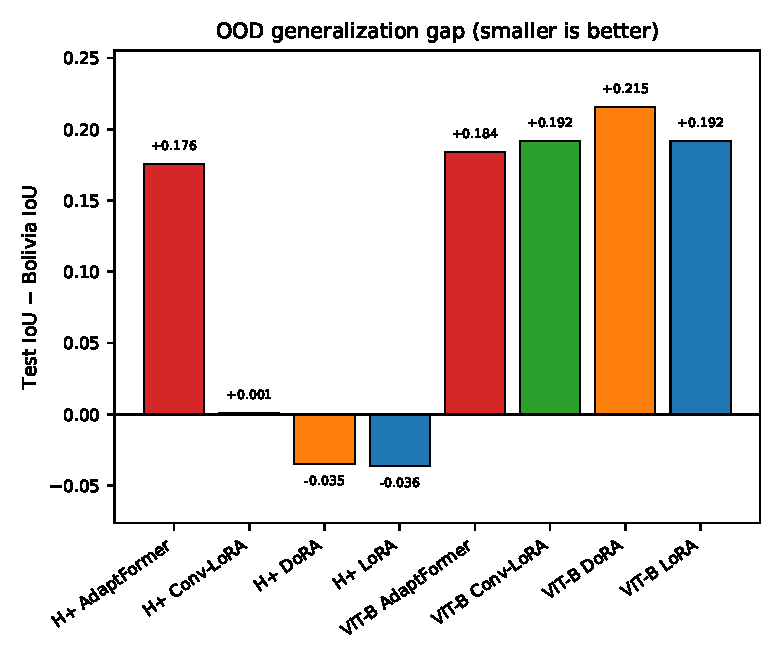
\includegraphics[width=\linewidth]{figs/ood_gap.pdf}}
  {\fbox{\parbox{0.8\linewidth}{\centering Figure pending sweep completion.}}}
\caption{Out-of-distribution generalization gap (in-distribution IoU minus Bolivia IoU) per method. Smaller indicates better generalization.}
\label{fig:ood_gap}
\end{figure}

\subsection{Discussion}
\label{sec:discussion}

We organize the discussion around the three gaps motivated in Section~\ref{sec:related} and the polarimetric ablation that surfaced the principal Pakistan-2022 OOD failure mode, reporting for each what the present paper does and does not settle.

\paragraph{PEFT comparison and the accuracy-vs-generalization trade-off}
AdaptFormer on SAM~2 Hiera-Base-Plus is the strongest single in-distribution choice, with $0.634 \pm 0.012$ IoU averaged across three seeds. The margin over the next-best PEFT method on the same backbone (DoRA at $0.602$) is $0.032$ IoU points; the margin over the U-Net baseline is $0.033$ IoU points. The LoRA family (LoRA, DoRA, Conv-LoRA) clusters within $0.003$ IoU of each other on SAM~2 Hiera-Base-Plus, and the statistical-significance analysis of Section~\ref{sec:results-stats} confirms small effect sizes ($|d_z| < 1.1$) within that cluster and large effect sizes ($|d_z| > 1.9$) between the cluster and AdaptFormer. The OOD-gap analysis of Section~\ref{sec:results-ood} reverses the picture: AdaptFormer on Hiera-Base-Plus has a Bolivia gap of $0.176$ and a Pakistan-2022 gap of $0.544$, while DoRA on the same backbone has a Bolivia gap of $-0.035$ (slight gain) and a Pakistan-2022 gap of $0.470$. The strongest in-distribution PEFT method is therefore not the most generalization-robust one; the LoRA family is preferable when held-out-country robustness matters. This documented trade-off is a substantive contribution that prior single-method SAM-for-SAR work~\cite{Pu2025CWSAM} could not surface.

\paragraph{Operational utility of aggregate-calibrated uncertainty}
The confidence-aware mechanism yields low expected calibration error on the headline cell ($0.053$ in-distribution test, $0.082$ Bolivia, $0.115$ Pakistan subset), with the reliability diagram of Figure~\ref{fig:reliability} tracking the diagonal. By the canonical ECE metric, the mechanism produces calibrated marginal probabilities. The selective-prediction curves of Section~\ref{sec:results-selective}, however, are flat on both out-of-distribution splits: abstaining on the most-uncertain pixels does not lift the IoU on the remainder. Aggregate calibration therefore does not imply that per-pixel uncertainty correctly ranks pixels by difficulty on OOD events. This is a negative finding, but it is the substantive content of the second gap: practitioners deploying SAR-flood models in humanitarian pipelines should not assume that a low-ECE estimator is operationally useful for selective prediction on previously unseen flood events. Sharper uncertainty estimators (deep ensembles, learned reject heads, epistemic-only decompositions) are required.

\paragraph{A public temporal-and-geographic OOD evaluation surface}
The Pakistan-2022 test set built in this work is, to our knowledge, the first 39-chip SAM-evaluation surface that pairs the publicly released TU Wien Sentinel-1 flood-extent product~\cite{Roth2023Pakistan} with Microsoft Planetary Computer Sentinel-1 RTC imagery via a documented acquisition pipeline at Sentinel-1's native 10-metre resolution. The released codebase covers the full pipeline (STAC search, native-resolution reading, nearest-neighbour mask upsampling, tiling), enabling reproducible foundation-model evaluation on a 2022 flood event that is strictly out-of-distribution to Sen1Floods11 in both time and geography. The Pakistan-2022 numbers throughout Section~\ref{sec:results} use this artifact.

\paragraph{Polarimetric composition and the Pakistan-2022 OOD failure mode}
The ratio and difference compositions are statistically indistinguishable (by the dB-domain identity they are mathematically equivalent inputs; point estimates differ by at most $0.006$, well within seed variance), and both beat the single-polarization control by $0.085$ IoU on the in-distribution test split and $0.104$ on Bolivia. On Pakistan-2022 the picture inverts dramatically. Across three seeds per cell, the single-polarization variant reaches $0.632 \pm 0.057$ IoU on Conv-LoRA, $0.631 \pm 0.050$ on LoRA, $0.658 \pm 0.014$ on DoRA, and $0.556 \pm 0.050$ on AdaptFormer (Table~\ref{tab:polari_pi}); the dual-polarization counterparts on the same PEFT methods sit between $0.092$ and $0.144$. None of the per-cell single-polarization confidence intervals overlap the dual-polarization band. Removing the cross-polarization channel therefore restores every SAM-family PEFT cell to within $0.01$ to $0.12$ of the U-Net Pakistan-2022 baseline ($0.672$), shrinking the OOD collapse to a small residual rather than eliminating it entirely. We read this as a falsifiable diagnosis of the failure mode: the cross-polarization channel encodes a feature whose marginal statistics shift on the Pakistan-2022 acquisition (different scattering geometry, different surface conditions, or different acquisition mode parameters between the Sen1Floods11 training distribution and August--September~2022 over Pakistan), and the adapted SAM image encoder amplifies that shift in a way the convolutional U-Net does not. Three implications follow. First, the in-distribution gain from dual-polarization is real but is acquisition-specific; it does not transfer to a 2022 Pakistan event drawn from the same nominal Sentinel-1 mission. Second, the AdaptFormer Pakistan-2022 single-pol mean ($0.556 \pm 0.050$) is meaningfully lower than the LoRA-family single-pol means ($0.63$ to $0.66$), suggesting AdaptFormer overfits to the in-distribution polarimetric statistics in a way that LoRA-style additive low-rank updates do not; the gap is approximately $1.5$ to $2$ standard deviations and is supported by three independent seed runs. Third, an operational SAR-flood pipeline that targets unseen regions or events should consider abstaining from the cross-polarization channel rather than relying on dual-polarization training. We flag the cross-pol distribution shift itself as a target for further investigation: characterizing whether it traces to incidence angle, sensor mode, surface scattering regime, or radiometric processing differences would convert this finding from a robust empirical claim to a calibrated cause-and-effect.

Three observations require honest reporting. First, AdaptFormer is the largest PEFT method in the comparison at $1.48$~M trainable parameters versus $0.60$~M for LoRA, and its IoU-per-million-parameter efficiency drops to $0.41$ from LoRA's $0.94$ (a $0.53$~IoU/M penalty), so its in-distribution win is not a free lunch on the parameter axis. Second, the Pakistan-2022 acquisition pipeline went through two acquisition-side fixes during the build: an initial Sentinel-1 RTC nodata-masking issue (anonymous-SAS no-coverage pixels surviving the $\texttt{(data==0)}$ check), and a resolution mismatch in which the original chips were built at the TU Wien 20-metre grid rather than the Sentinel-1 native 10-metre grid; the results in Table~\ref{tab:results_main} use the third-round pipeline that keeps Sentinel-1 imagery at native 10~m, reprojects the TU Wien masks upward via nearest-neighbour, and applies a $-50$~dB ignore threshold on the Pakistan-2022 split. The aggregate JSON file in the released codebase includes the pre-patch numbers under a $\texttt{before\_v2}$ backup. Third, an early bug in AdaptFormer initialization (scale and up-projection both zero, freezing the side-path forever) was caught mid-build and fixed before the Vast.ai sweep; the recovery and the trace of the cleaner-vs-logger race are documented in the supplementary incident log accompanying the released codebase.

% --- 7. Conclusion ---
\section{Conclusion and Future Work}
\label{sec:conclusion}

This paper has presented the design, implementation, and empirical evaluation of a parameter-efficient adaptation of SAM~2 to Sentinel-1 SAR flood inundation mapping, addressing three substantive gaps in prior work. The systematic head-to-head PEFT comparison documents an accuracy-vs-generalization trade-off that single-method prior work could not surface: AdaptFormer maximizes in-distribution IoU on SAM~2 Hiera-Base-Plus ($0.634$), while the LoRA family is the more generalization-robust choice on held-out countries. The polarimetric ablation localizes the Pakistan-2022 OOD failure mode to the cross-polarization channel itself: across three seeds per single-polarization cell, removing the cross-polarization channel restores every SAM-family PEFT cell from a $0.09$ to $0.14$ IoU floor to a $0.56$ to $0.66$ IoU regime ($\pm$ $0.014$ to $0.057$ standard deviation), within $0.01$ to $0.12$ IoU of the U-Net baseline at $0.672$. The dual-level uncertainty evaluation produces a substantive negative finding: aggregate calibration (ECE $0.053$ in-distribution) does not imply useful per-pixel uncertainty on out-of-distribution flood events, which the flat selective-prediction curves expose. The released Pakistan-2022 test set provides the first 39-chip SAM-evaluation surface combining temporal and geographic out-of-distribution shift via a documented acquisition pipeline that matches Sentinel-1's native 10-metre resolution. The full experimental sweep, spanning five backbones, four PEFT methods, three random seeds, polarimetric ablations, a U-Net baseline and zero-shot baselines, completes in approximately 3.5 hours on a dual NVIDIA RTX PRO 5000 Blackwell cloud instance for under ten US dollars of cloud compute.

We document seven limitations honestly.

\textit{(1) Stretch backbones under Conv-LoRA only.} The three larger backbones (ViT-L, ViT-H, Hiera-Large) are evaluated only under Conv-LoRA rather than the full PEFT cross-product. Whether AdaptFormer would further close the gap on Hiera-Large, or whether a tuned learning rate would recover SAM ViT-H, is left to future replications with a larger compute budget.

\textit{(2) SAM~2 memory module disabled.} The streaming memory module is included in the codebase but disabled in the principal evaluation, because the Sen1Floods11 hand-labeled chips are single-frame rather than bi-temporal. An empirical comparison between memory-on and memory-off variants is left to future work that pairs each chip with a pre-event reference.

\textit{(3) Bangladesh-Sylhet pipeline shipped but not evaluated.} A standalone construction pipeline for a Bangladesh-2022-Sylhet test set, targeting the June~2022 monsoon flood event, is released alongside the codebase but its chips are not empirically evaluated here. Closing the regional-generalization question on Bangladesh deltaic conditions is the most immediate direction for future work.

\textit{(4) Ratio and diff polarimetric compositions are mathematically equivalent.} By the identity $\log_{10}(P_{VV}/P_{VH})\cdot 10 = (VV)_{dB} - (VH)_{dB}$, the two definitions in Section~\ref{sec:results-polari} produce identical numerical inputs. The meaningful contrast is therefore between dual-pol (ratio or diff, treated equivalently) and single-pol; a genuinely distinct diff implementation in linear power is left to future replication.

\textit{(5) Pakistan-2022 labels are not fully independent ground truth.} The evaluation rests on $39$ chips and on TU Wien labels that were themselves derived from a Sentinel-1-based segmentation pipeline~\cite{Roth2023Pakistan}, not from independent ground truth. The U-Net baseline's $0.672$ Pakistan-2022 IoU, which essentially matches its Bolivia held-out IoU, is therefore partially explained by methodological similarity between the TU Wien label-generation pipeline and the convolutional baseline. The absolute IoU level on Pakistan-2022 should be read relative to the in-table baseline rather than as a fully independent measurement; the relative ordering between dual-polarization SAM-family cells, single-polarization SAM-family cells, and U-Net is the substantive comparison and is robust to this caveat.

\textit{(6) Pakistan-S1F11 subset is too small.} The 12-chip regional in-distribution slice, drawn entirely from the 2010 event, produces noticeably lower IoU than the corresponding Bolivia split across every cell including the U-Net baseline ($0.271$ versus $0.684$). We attribute this to small-sample variance and the specific scene composition of the 2010 chips, and document the discrepancy so that readers do not over-interpret the Pakistan-S1F11 column as an in-distribution-quality estimate.

\textit{(7) Pakistan-2022 acquisition history (two iterative fixes).} The pipeline went through two acquisition-side rebuilds during this work. Round-one chips revealed that the nodata mask was incomplete: Microsoft Planetary Computer Sentinel-1 RTC encodes weak-coverage pixels as tiny positive linear values that the original \texttt{(data==0)} check missed, leaving $-100$~dB pixels in chips after the \texttt{linear\_to\_db} clamp. This was patched by broadening the nodata mask and by adding a split-specific $-50$~dB ignore threshold in the dataset loader (preserving checkpoint compatibility on the Sen1Floods11 splits). Round-two chips were built at the TU Wien $20$~m Equi7Grid rather than Sentinel-1's native $10$~m, introducing a resolution mismatch with the Sen1Floods11 training distribution. The pipeline was rebuilt to keep Sentinel-1 at native $10$~m and to reproject the TU Wien masks upward via nearest-neighbour, producing $39$ chips. The round-three pipeline used in this paper is the only variant whose results are reported in the present tables; the pre-patch aggregate is preserved as a \texttt{before\_v2} backup file in the released codebase for traceability.

\section*{Acknowledgment}

Sentinel-1 imagery is provided by the European Space Agency under the Copernicus open and free data policy. Sentinel-1 Radiometric Terrain Corrected products are made available by Microsoft Planetary Computer. Pakistan-2022 flood-extent labels are released by TU Wien under CC-BY 4.0~\cite{Roth2023Pakistan}.

% --- Bibliography ---
\begin{thebibliography}{00}

\bibitem{Kirillov2023SAM}
A.~Kirillov \textit{et al.}, ``Segment Anything,'' in \textit{Proc. IEEE/CVF Int. Conf. Comput. Vis. (ICCV)}, 2023, pp.~4015--4026.

\bibitem{Ravi2025SAM2}
N.~Ravi \textit{et al.}, ``SAM 2: Segment Anything in Images and Videos,'' in \textit{Proc. Int. Conf. Learn. Represent. (ICLR)}, 2025.

\bibitem{Hu2022LoRA}
E.~J. Hu \textit{et al.}, ``LoRA: Low-Rank Adaptation of Large Language Models,'' in \textit{Proc. Int. Conf. Learn. Represent. (ICLR)}, 2022.

\bibitem{Liu2024DoRA}
S.-Y. Liu \textit{et al.}, ``DoRA: Weight-Decomposed Low-Rank Adaptation,'' in \textit{Proc. Int. Conf. Mach. Learn. (ICML)}, 2024.

\bibitem{Zhong2024ConvLoRA}
Z.~Zhong \textit{et al.}, ``Convolution Meets LoRA: Parameter Efficient Finetuning for Segment Anything Model,'' in \textit{Proc. Int. Conf. Learn. Represent. (ICLR)}, 2024.

\bibitem{Chen2022AdaptFormer}
S.~Chen \textit{et al.}, ``AdaptFormer: Adapting Vision Transformers for Scalable Visual Recognition,'' in \textit{Adv. Neural Inf. Process. Syst. (NeurIPS)}, 2022.

\bibitem{Ma2024MedSAM}
J.~Ma, Y.~He, F.~Li, L.~Han, C.~You, and B.~Wang, ``Segment Anything in Medical Images,'' \textit{Nat. Commun.}, vol.~15, no.~1, p.~654, 2024.

\bibitem{Saleh2024DAMNet}
T.~Saleh, X.~Weng, S.~Holail, C.~Hao, and G.-S. Xia, ``DAM-Net: Flood Detection from SAR Imagery Using Differential Attention Metric-Based Vision Transformers,'' \textit{ISPRS J. Photogramm. Remote Sens.}, vol.~212, pp.~440--453, 2024.

\bibitem{Bonafilia2020Sen1Floods11}
D.~Bonafilia, B.~Tellman, T.~Anderson, and E.~Issenberg, ``Sen1Floods11: A Georeferenced Dataset to Train and Test Deep Learning Flood Algorithms for Sentinel-1,'' in \textit{Proc. IEEE/CVF Conf. Comput. Vis. Pattern Recognit. Workshops (CVPRW)}, 2020, pp.~210--211.

\bibitem{Pu2025CWSAM}
X.~Pu, H.~Jia, L.~Zheng, F.~Wang, and F.~Xu, ``ClassWise-SAM-Adapter: Parameter-Efficient Fine-Tuning Adapts Segment Anything to SAR Domain for Semantic Segmentation,'' \textit{IEEE J. Sel. Top. Appl. Earth Obs. Remote Sens.}, vol.~18, pp.~4791--4806, 2025.

\bibitem{Sharma2025DeepSARFlood}
N.~K. Sharma and M.~Saharia, ``DeepSARFlood: Rapid and Automated SAR-Based Flood Inundation Mapping Using Vision Transformer-Based Deep Ensembles with Uncertainty Estimates,'' \textit{Sci. Remote Sens.}, vol.~11, p.~100203, 2025.

\bibitem{Hu2025GlobalFloods}
B.~Hu \textit{et al.}, ``Mapping Global Floods with Ten Years of Satellite Radar Data,'' \textit{Nat. Commun.}, 2025.

\bibitem{Marsocci2024PANGAEA}
V.~Marsocci \textit{et al.}, ``PANGAEA: A Global and Inclusive Benchmark for Geospatial Foundation Models,'' \textit{arXiv preprint arXiv:2412.04204}, 2024.

\bibitem{Roth2023Pakistan}
F.~Roth, B.~Bauer-Marschallinger, M.~Tupas, C.~Reimer, P.~Salamon, and W.~Wagner, ``Sentinel-1-based Analysis of the Severe Flood over Pakistan 2022,'' \textit{Nat. Hazards Earth Syst. Sci.}, vol.~23, pp.~3305--3317, 2023.

\end{thebibliography}

\end{document}
